	
% This template was initially provided by Dulip Withanage.
% Modifications for the database systems research group
% were made by Conny Junghans,  Jannik Strötgen and Michael Gertz

\documentclass[enabledeprecatedfontcommands,
     12pt,         % font size
     a4paper,      % paper format
     BCOR10mm,     % binding correction
     DIV14,        % stripe size for margin calculation
%     liststotoc,   % table listing in toc
%     bibtotoc,     % bibliography in toc
%     idxtotoc,     % index in toc
%     parskip       % paragraph skip instad of paragraph indent
     ]{scrreprt}

%%%%%%%%%%%%%%%%%%%%%%%%%%%%%%%%%%%%%%%%%%%%%%%%%%%%%%%%%%%%

% PACKAGES:

% fix bitmap fonts
\usepackage{lmodern}
% Use German :
\usepackage[ngerman,english]{babel}
\usepackage{amsmath}
% Input and font encoding
\usepackage[latin1]{inputenc}
\usepackage[T1]{fontenc}
% Index-generation
\usepackage{makeidx}
% Einbinden von URLs:
\usepackage{url}
% Special \LaTex symbols (e.g. \BibTeX):
%\usepackage{doc}
% Include Graphic-files:
\usepackage{graphicx}
% Include doc++ generated tex-files:
%\usepackage{docxx}
% Include PDF links
%\usepackage[pdftex, bookmarks=true]{hyperref}

% Fuer anderthalbzeiligen Textsatz
\usepackage{setspace}

% hyperrefs in the documents
\usepackage[bookmarks=true,colorlinks,pdfpagelabels,pdfstartview = FitH,bookmarksopen = true,bookmarksnumbered = true,linkcolor = black,plainpages = false,hypertexnames = false,citecolor = black,urlcolor=black]{hyperref} 
%\usepackage{hyperref}

%%%%%%%%%%%%%%%%%%%%%%%%%%%%%%%%%%%%%%%%%%%%%%%%%%%%%%%%%%%%

% OTHER SETTINGS:

% Pagestyle:
\pagestyle{headings}

% Choose language
\newcommand{\setlang}[1]{\selectlanguage{#1}\nonfrenchspacing}
\newcommand*\mean[1]{\bar{#1}}
\begin{document}

% TITLE:
\pagenumbering{roman} 
\begin{titlepage}


\vspace*{1cm}
\begin{center}
\vspace*{3cm}
\textbf{ 
\Large Heidelberg University\\
\smallskip
\Large Institute of Computer Science\\
\smallskip
\Large Visual Computing Group (VCG)\\
\smallskip
}

\vspace{3cm}

\textbf{\large Master-Arbeit} % Bachelor-Arbeit 

\vspace{0.5\baselineskip}
{\huge
\textbf{Light Transport Techniques for Tensor Field Visualization}
}
\end{center}

\vfill 

{\large
\begin{tabular}[l]{ll}
Sebastian Bek\\
Matrikelnummer: & 3481802\\
Betreuer: & Sebastian Bek\\
Datum der Abgabe: & 07.07.2019
\end{tabular}
}

\end{titlepage}

\onehalfspacing

\thispagestyle{empty}

\vspace*{100pt}
\noindent
\emph{dt.:}
Ich versichere, dass ich diese Master-Arbeit selbstst�ndig verfasst und nur die angegebenen
Quellen und Hilfsmittel verwendet habe und die Grunds�tze und
Empfehlungen ``Verantwortung in der Wissenschaft'' der Universit�t Heidelberg beachtet wurden. 
\bigskip
\\
\emph{eng.:}
I hereby declare/assure, that I drafted this thesis independently and only used the sources and materials labeled as references and that the conventions/principles and recommendations ``Verantwortung in der Wissenschaft'' of the Heidelberg University have been regarded/observed. 
\vspace*{50pt}
\noindent

\underline{\phantom{mmmmmmmmmmmmmmmmmmmm}}

\medskip
\noindent 
Abgabedatum / Due Date: 07.07.2019
\newpage

% Add a brief summary of your topic and contributions (Zusammenfassung) in German *and* in English:
\chapter*{Zusammenfassung}
%
% This file contains the German version of your abstract, with about 300-500 words

Die Zusammenfassung muss auf Deutsch \textbf{und} auf Englisch geschrieben
werden. Die Zusammenfassung sollte zwischen einer halben und einer
ganzen Seite lang sein. Sie soll den Kontext der Arbeit, die
Problemstellung, die Zielsetzung und die entwickelten Methoden sowie
Erkenntnisse bzw.~Ergebnisse �bersichtlich und verst�ndlich
beschreiben.

Tensorfelder werden meistens in Verbindung mit mechanischen Spanunngsverteilungen in 2D/3D-Gittern gebracht (vgl. Cauchy-Stress Tensor), haben aber auch andere praktische Bedeutungen in der Physik.
Mithilfe von globalen Beleuchtungsmodellen/-techniken wird eine neue Methode entwickelt, um Tensorfelder zu visualisieren, die aber zus�tzlich auch verwendet werden kann um die Lichtausbreitung in einer topologischen Szene zu beschreiben. Als Grundlage leiten wir ein einfaches Lichtausbreitungsschema f�r kartesische Gitter ab, dass die Prinzipien der Ausbreitungsd�mpfung und Energieerhaltung beachtet und Licht-verteilung/en f�r gegebene Lichtquellenrichtung/en und -positionen bis zur Konvergenz approximieren kann. Als unterliegendes Modell werden die Transmissionsprofile innerhalb diesem Gitter als Kristallfiberstruktur angenommen (vgl. Edelsteine: Katzenaugeneffekt beim Tigerauge). Die folgende Aufgabe ist es, anisotrope Fiberstrukturen mit der Orientierung und den Anisotropiema�en des unterliegenden Tensorfelds zu modellieren. Daf�r erstellen wir per Hauptachsentransformation (PCA) ein Eigensystem f�r jede Zelle des Tensorfelds und modellieren eine zugeh�rige Ellipsengleichung als (Transfer-/Wichtungs-) Transmissionsprofil. Folglich kann die resultierende Lichtverteilung als 2D Skalarfeld oder Polarplots f�r Richtungsinformation visualisiert/repr�sentiert werden. Wir messen Impulsantworten des Tensorfelds mit Delta-Pulsen an jeder Position und in jede Richtung um eine uniform gesamplete Map der globalen Lichtverteilungen zu erhalten. Diese Map wird als ein globales Energieflussfeld betrachtet. Wir lassen uns von der Technik FTLE aus dem Bereich Particle Tracing der Vector Field Visualization inspirieren, indem wir den Gradient des Flussfelds der resultierenden Lichtverteilungen analysieren und visualisieren. �hnlich wie FTLE in Vektorfeldern Gr�te/K�mme/LCS detektiert, erfasst unsere Methode dieselben Strukturen, anziehende/absto�ende/sattelnde Tensorfeldlinien die h�ufig Schl�sselstrukturen in der Natur repr�sentieren, in Tensorfeldern. Wir f�hren diese Gr��e als Global Illumination Gradient ein, der einen FTLE-verwandten Ansatz darstellt, um LCS in Tensorfeldern durch die Analyse des globalen, durch einen Imprint (Gravur in kristallinen Fiberstrukturen) gerichteten Lichtflusses, zu visualisieren.
\newpage

\chapter*{Abstract}
%
% This file contains an abstract of your thesis, with approximaltely 300-500 words

The abstract has to be given in German \textbf{and} English. It should
be between half a page and one page in length. It should cover in a
readable and comprehensive style the context of the thesis, the
problem setting, the objectives, and the methods developed in this
thesis as well as key insights and results.

Tensor fields, are most commonly associated with stress distributions (cf. Cauchy-stress tensor) in 2D/3D grids, but also have some other meanings in practice in physics. By means of global illumination techniques, we motivate a new method to visualize tensor fields, which is also capable of visualizing the light transport (propagation) in a topologically defined scene geometry. As a basis, we derive a simple light propagation scheme for Cartesian grids, which satisfies propagation attenuation and energy-conservation principles and is able to approximate light distributions for given light source position(s) and direction(s) until convergence. The transmission profiles within this grid are considered as crystal fiber structures as an underlying physical model (eg. gemstones: tiger's eye's cat's eye effect). The consequent task is to model anisotropic fibre structures with the orientation and anisotropy measures of the underlying tensor field in the grid.
For this, we derive an eigenbasis by PCA (principal component analysis) for every cell of the tensor field and form an ellipsoid equation as transmission (transfer/weighting) function for the transmitted light profiles. Hence, the resulting light distribution can be visualized via 2D scalar field or polar plots for directional information. Additionally, We measure impulse responses of the tensor field with Dirac-pulses as light sources at any (sampled) position and in any direction to generate a uniform sampled map of the global illumination distributions. This map is considered as a global illumination energy flow field.
We gain inspiration by vector field particle tracing's FTLE approach for analyzing the gradient of the flow field of the resulting light distributions. Similar to how the FTLE detects ridges/LCS (Lagrangian coherent structures) in vector fields (flow fields), our approach captures these structures likewise, attracting/repelling/saddling tensor field lines (TFL) which frequently represent key structures in nature, in tensor fields. We denote this entity a global illumination gradient which states an FTLE-related approach for visualizing LCS in tensor fields through analysis of the global and light transport  directed by imprint/engraving in crystelline fiber structures modeled by the tensor field's ellipsoid glyhps. We evaluate our approaches for plausibility and comparability within an extensive test campaign and demonstrate its performance on several examples of datasets.
\newpage

% MAIN PART:
% Table of contents (Inhaltsverzeichnis)
\tableofcontents
\cleardoublepage
\pagenumbering{arabic} 

% List of figures (Abbildungsverzeichnis):
%\listoffigures
% List of tables (Tabellenverzeichnis):
%\listoftables

%%%%%%%%%%%%%%%%%%%%%%%%%%%%%%%%%%%%%%%%%%%%%%%%%%%%%%%%%%%%%%%
% Here, the actual content of your thesis begins
% You can either put all the text here or use individual files to store the chapters of your thesis.
% Below are templates for both alternatives.

\chapter{Introduction}\label{intro}

In this work, we will discuss the advantages of tensor field analysis and motivate a new method for tensor field through a coherent light transport visualization. At first, we will shortly state the problem setting objectives and then give a quick overview about the structure of this work.

\paragraph{Contributions of this Work}
\begin{itemize}
	\item Motivation of a light transport technique following basic but crucial physical principles for tensor field visualization
	\item Design of a FTLE-related approach for visualizing key structures (ROIs) in $2D$ second-order tensor fields
	\item Discussion of the proposed techniques in the context of other works in this field
\end{itemize}
%Dieses Kapitel gibt einen �berblick �ber die Arbeit. Gerade der
%Abschnitt zur Motivation soll allgemein verst�ndlich geschrieben
%werden. Die Einleitung sollte auch wichtige Referenzen enthalten. 

\section{Motivation}
\label{sect:motiv}
Tensor Field Visualization is gaining importance as a relevant tool for the analysis of fluid and solid mechanics. Tensors are found most commonly in medical, scientific and engineering applications. A tensor is a $n$-D generalization of a matrix and appears, e.g., as Jacobian-Matrix in vector (Flow) field visualization or as stress tensor in solid continuum mechanics. Basically, tensors describe compressions, tensions, rotations and volume changes in both solid and fluid material. While most techniques focus on symmetric tensor field visualization (like glyphs and tensor field lines), some other recent works adress the problem of asymmetric tensor field visualization. The issue with asymmetric or antisymmetric tensors is that they do not always yield real eigenvalues, which is needed to determine an eigenbasis to set up glyphs, hyperstreamlines or tensor field lines. \cite{pang&zheng} Zheng \& Phang et al. proposed the concept of dual eigenvectors and \cite{zhang} Lin et al. extended it to pseudo-eigenvectors and introduced eigenvector and eigenvalue manifold to visualize eigenvectors in the complex domain. In this work, we will use the $\mathbf{U}$-matrix obtained from singular value decomposition (SVD) to obtain the half-axes of the PCA principal ellipsoid as suggested by Moler \cite{moler}.\\


\begin{figure}[!t]
  \centering
 {
    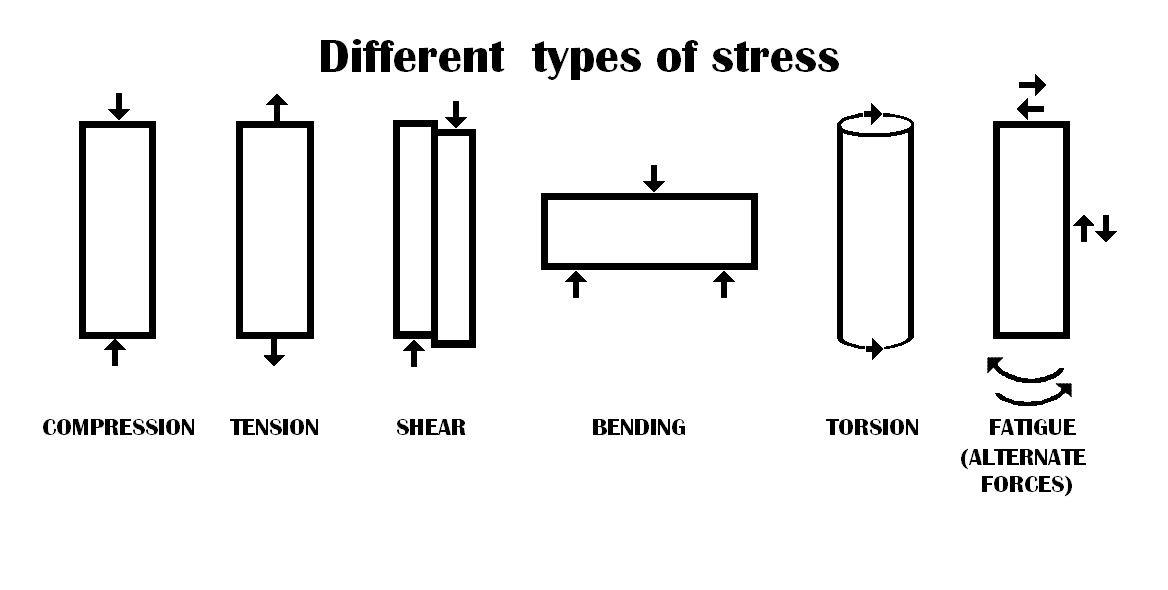
\includegraphics[width=0.6\textwidth]
    {img/DIFFERENT_TYPES_OF_STRESS.png}
  }
  \caption{Different types of stress}
  \label{Skalierung}
\end{figure}


Worum geht es? Beispiel(e)! Illustrationen sind hier meist sinnvoll
zum Verst�ndnis. Warum ist das Thema wichtig? In welchem Kontext?

\section{Objectives}
\begin{figure}[!t]
  \centering
 {
    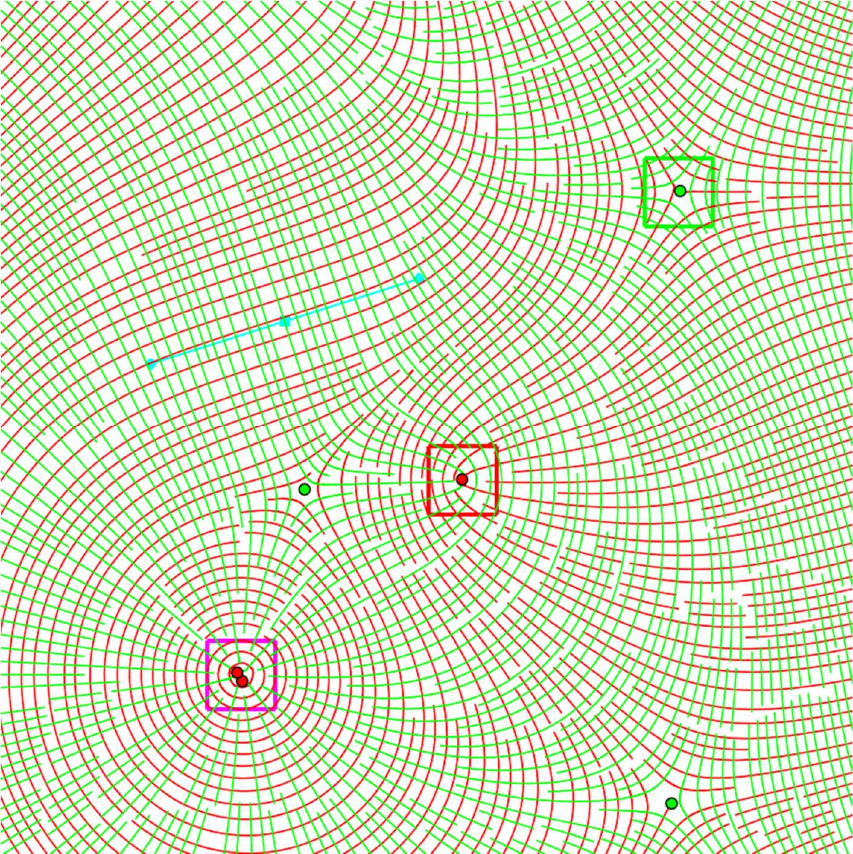
\includegraphics[width=0.6\textwidth]
    {img/hyperstreamlines.png}
  }
  \caption{Hyperstreamlines in Tensor Field Visualization}
  \label{Skalierung}
\end{figure}
The main purpose of visualization in general is to reduce or encode some set of numbers in some readable, explorable and more intuitive representation. This implies, e.g., clustering, structuring or projection techniques. When it comes to tensor fields, this comes handy in, e.g., medical sciences such as in DT-MRI (diffusion tensor-medical resonance imaging) or in simulated (or measured) stress tensor fields from solid and fluid mechanics. The problem setting encomprises the visualization of tensor fields, i.e., mostly 2D/3D-grids consisting of mainly second-order tensors (cf. Cauchy-Stress Tensor) with the additional possibility to model light transport transport in a geometrical scene. The objective of this work is to design a simple light propagation scheme following the most basic but crucial physical principles and laws. This propagation scheme can either be used to visualize the light transport paths (separatrices) in a scene defined by geometry. Or, on the other hand, be used to visualize the anisotropy characteristics of a given tensor field. Therefore the tensor field somehow needs to be pre-processed to generate a tensor-induced footprint map of transmission profiles. Hence however, the tensors need to be decomposed to obtain a kind of transmission profile. Another aim is to implement an approach borrowed from vector-field visualization. We construct an FTLE-related approach in tensor field visualization (both symmetric and asymmetric) for detecting ridges/LCS (Lagrangian coherent structures). These structures can be classified (identified) as repelling, attracting and saddling (forming a saddle) local features, which frequently represent key structures in nature. LCS usually separate regions of different flow behavior, but in our case they separate regions/domains of varying directional distributions (w.r.t. direction/location) represented by tensors. The map responds most where tensor field lines / hyperstreamlines converge or diverge, whereas one is the same as the other because of bidirectional stress directions and since we effectively measure the FTLE with both forward and backward integration time (stimulus directions). The real part of the eigenvalues could be exploited for sign change (contractions/tensions) which leads to the concept of deformation glyphs w. attached arrows pointing inward/outward for the two types of normal stresses. Practically, in its eigenbasis there are no shear stresses existent for the symmetric stress tensor in equilibrium, just the principal normal stresses. Thus, we can even define the full set of stresses with the glyphs which are derived from the singular value decomposition and signed with the real part of the eigenvalues (in corresponding absolute order). The main goal of this work is therefore the encoding of a tensor field into certain elaborate representations and the interpretation of meaningful results comparing the proposed techniques against each other. The designed approach could e.g. be applied in medicinal sciences, engineering and physics to reveal structures which are hard to grasp through interpreting simpler glyph and tensor field line visualizations.


%In diesem Abschnitt sollen neben den Herausforderungen und der
%Problemstellung insbesondere die Ziele der Arbeit beschrieben werden. 

\section{Structure of this Work}
 
For the rest of this work, we will give a quick overview on the structure and outline. Next, in chap. \ref{chap:grundlagen}, we will capture important fundamentals like Tensors and PCA in the context of singular value decomposition (generalization of eigenvalue decomposition). Also we will discuss the most relevant related work in the domain of tensor field visualization. In chap. \ref{chap:main} we will propose the main contributions of this work and document the experimental evaluation in chap. \ref{chap:eval}. A compact Summary, Conclusion and Outlook will be given in chap. \ref{chap:concl}.\\

%Dieser Abschnitt wird meist recht kurz gehalten und beschreibt im
%Prinzip nur den Aufbau des Rests der Arbeit. Zum Beispiel: In Kapitel
%\ref{chap:grundlagen} geben wir einen �berblick �ber die  Grundlagen
%zu der Arbeit sowie �ber verwandte Arbeiten. In Kapitel
%\ref{chap:main} stellen wir dann \ldots vor. \ldots etc.

%%%%%%%%%%%%%%%%%%%%%%%%%%%%%%%%%%%%%%%%%%%%%%%%%%%%%%%%%%%%


\chapter{Fundamentals and Recent Work}
\label{chap:grundlagen}

In this chapter, we will capture the prerequisites necessary to understand the contributions of this work and will capture Tensors, PCA, GT approaches and Related Work in that sense.

%Die ersten paar Abschnitte in diesem Kapitel f�hren in die Grundlagen
%zur Arbeit ein. Das k�nnen beispielsweise Grundlagen zu Netzwerken
%oder zur Informationsextraktion sein. 

\section{Tensor Fields}
\label{sec:tensors}
Now what is a Tensor? A tensor is a $o$-dimensional generalization of a matrix as illustrated in Table \ref{tensor}.
\begin{table}[!b]
\centering
\caption{Tensor Shapes}
 \begin{tabular}{c|c|c|c|c|c|c}
\textbf{order} & 0 & 1 & 2 & 3 & ... & o \\ 
\hline 
\textbf{shape} & scalar & vector & matrix & ``3D-matrix'' & ... & $\mathop{o}$D-matrix\\ 
\end{tabular}
\label{tensor}
 \end{table} 
In addition to that, a tensor has as many indices as its order $o$ and their run length is as long as its embedded dimension $n$ (the dimensin of the row and column vectors), which is equal to the rank of the tensor for full rank (or in other words the number of elements n for a $n{\times}n$-matrix). Tensors follow certain transformation rules which are defined for covariant/contravariant tensors. They are most commonly obtained and defined from physical transformation equations. Hence, any $o$-D number array could be a tensor, but the definition holds only if the transformation rules apply to these $o$-D number arrays (in a sense of physical interpretation), which is mostly true for component-indexed $o$-D number entities following matrix multiplication and transformation rules found in physics and math. In fact, tensors themselves are interpreted as a transformation which reflects an incoming direction vector (measuring, e.g., the stress in that direction) to an outgoing stress vector.
 To be a bit more concrete, tensors represent stress distributions in solids and fluids describing strain and flow features as these entities aren't simple numbers or vectors. They occur in form of a tensor fields, and thus as entities or quantities in physics. That is, at each point in space (indexed by the grid) there is a whole distribution of, e.g., stresses (elastic and viscous) which needs to be characterized and represented by a single tensor.
 \\
 \paragraph{stress tensor}
 \begin{figure}[!t]
  \centering
 {
    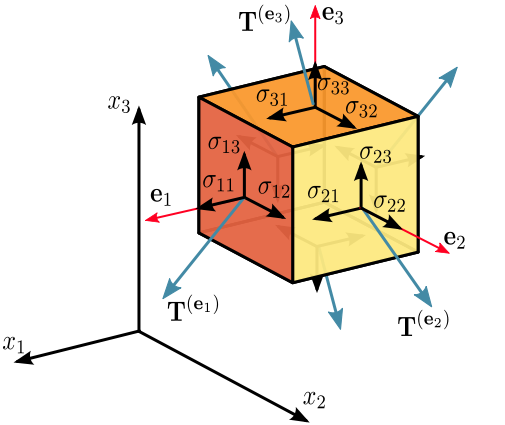
\includegraphics[width=0.6\textwidth]
    {img/stress_tensor.png}
  }
  \caption{Cauchy-Stress Tensor}
  \label{cauchy}
\end{figure}

The Cauchy stress tensor, which is propably the classical example of a tensor, is depicted in Fig. \ref{cauchy} and consists of 3 stress vectors $\mathbf{T(e_i)}$ arranged in row-major order. It appears in similar form as viscous stress tensor in fluid mechanics:
\begin{align*}
\boldsymbol{\sigma}
 = \left[{\begin{matrix} \mathbf{T}^{(\mathbf{e}_1)} \\
\boldsymbol{T}^{(\mathbf{e}_2)} \\
\boldsymbol{T}^{(\mathbf{e}_3)} \\
\end{matrix}}\right] =
\left[{\begin{matrix}
\sigma _{xx} & \sigma _{xy} & \sigma _{xz} \\
\sigma _{yx} & \sigma _{yy} & \sigma _{yz} \\
\sigma _{zx} & \sigma _{zy} & \sigma _{zz} \\
\end{matrix}}\right]  = \left[{\begin{matrix}
\sigma _x & \tau _{xy} & \tau _{xz} \\
\tau _{yx} & \sigma _y & \tau _{yz} \\
\tau _{zx} & \tau _{zy} & \sigma _z \\
\end{matrix}}\right] =
\begin{bmatrix}
\sigma _{11} & \sigma _{12} & \sigma _{13} \\
\sigma _{21} & \sigma _{22} & \sigma _{23} \\
\sigma _{31} & \sigma _{32} & \sigma _{33} 
\end{bmatrix}.
\end{align*}
These 3 stress vectors represent the orientation and magnitude of total resulting stress at plane ${x,y,z}$ in direction ${x,y,z}$ ($3^2=9$ individual numbers). Thus, the stress tensor poses a full valid represenation of the stress distribution at any point in space. The stress tensor itself can be interpreted as a transformation which maps an incoming normal direction vector $\mathbf{n}$ a resulting stress vector $\mathbf{T^{(n)}} = \mathbf{n}\cdot\boldsymbol{\sigma}$. The stresses in normal directions (diagonal elements) are directly related to the pressure, which is always isotropic and hence non-directionally dependent. It is possible to find 2 principal stress directions in 2D through PCA (see sect. \ref{sec:pca} below), for which there are no shear stresses existent in equilibrium. These form the principal directions of deformation at a certain location and are sufficient to describe the resulting transformation/deformation behaviour. The resulting system of principal directions and absolute stresses is often called an ``eigensystem'' or ``eigenframe''. So to say, an eigensystem, consistent of the principal directions/axes, spans a principal ellipsoid depicted in Fig. \ref{HAT} in sect. \ref{sec:pca}.
Another interpretation for the principal component ellipsoid is that it is the result of the tensor transformation applied to the unit circle. It is therefore somehow representing the distortion of an absolutely isotropic object (unit circle) by whatever the affine transformation effects (e.g. stretching, shearing, mirroring, scaling, rotating).
\section{Principal Component Analysis}
\label{sec:pca}
Note that we denote a matrix with a second order tensor interchangeably for the sake of simplicity in the following. For any state of stress in equilibrium it is possible to find $n$ (dimensionality) independent orthogonal directions with no shear stresses existent. Along these directions the principal stresses, which are normal (tensile/compressive) stresses, are exerted. The anisotropy can be represented by, e.g., ellipsoid glyphs.

\begin{figure}[!t]
%\centering
  \begin{minipage}{0.5\textwidth}
    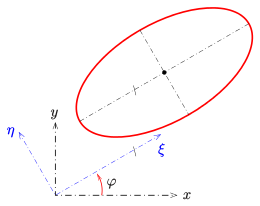
\includegraphics[width=\textwidth]{img/HAT.png}
    \label{HAT}
  \end{minipage}
  \begin{minipage}{0.5\textwidth}
    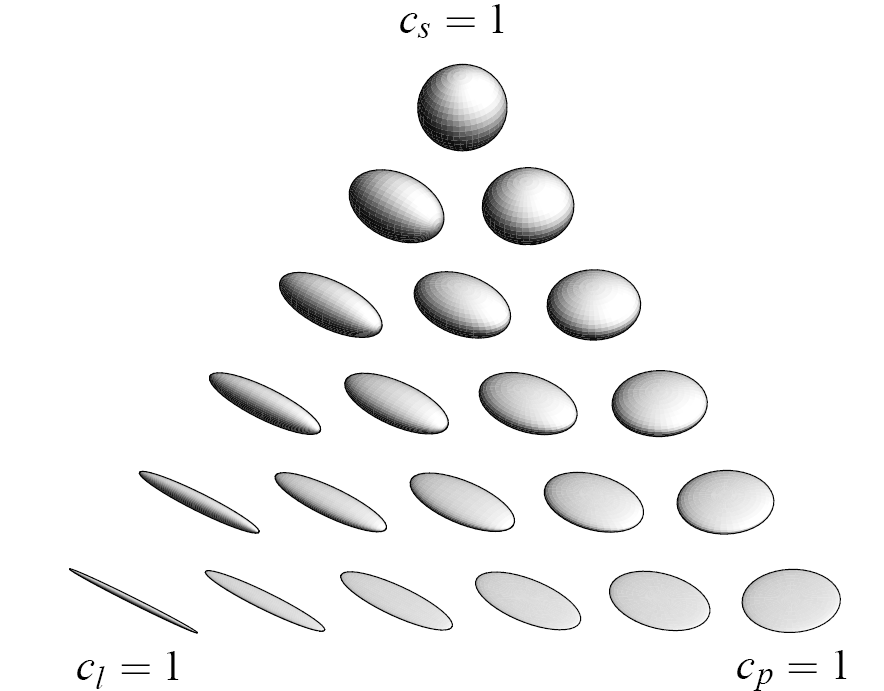
\includegraphics[width=\textwidth]{img/glyphs.png}
    \label{b)}
  \end{minipage}
\caption{a) 2D Principal component ellipsoid (eigenframe), b) 3D ellipsoid glyphs w. anisotropy coefficient (l:linear, p:planar, s:spherical)}
\label{gradient}
\end{figure}

Principal Component Analysis is an algorithm which can capture the principal components (directions) in stochastic data. But it works similarly on transformations to capture the principal directions from transformations like rotation and scaling. Now, principal component analysis can be done by eigenvalue or singular vector decomposition, whereas the former yields complex eigenvalues for asymmetric matrices. For (skew-)symmetric (normal) matrices, they are connected through the following relation: $s_i = \sqrt{|\lambda_i|}$ (cf. \cite{kieburg}). Note that the eigenvectors match the singular vectors only for symmetric matrices, which does not mean that they do not form the half-axes of the principal component ellipsoid in other cases. Mathematically speaking, a decomposition is somehow decomposing a transformation (which follows certain transformation rules) into parts of subsequent transformations consistent of rotation and scaling ($\mathbf{A} = \mathbf{R}\mathbf{S}\mathbf{R}^*$). We choose to use singular value decomposition ($\mathbf{A} = \mathbf{U} \mathbf{\Sigma} \mathbf{V}^*$) to be able to set up real eigenvalues for any kind of matrix (singular values are always real and positive). Also, the singular vectors of the $\mathbf{U}$-matrix represent the half-axes of the principal ellipsoid (eigenframe) shown in Fig. \ref{HAT} for any kind of matrix as pointed out by Moler \cite{moler}. In addition, we also calculate the eigenvalues to exploit the sign of the real part of the eigenvalues (\cite{mroz}) ordered decreasingly by absolute value (corresponding to singular value order). The sign corresponds to tensile ($+$) and compressive ($-$) stress, which would allow us to visualize deformation glyphs with arrows pointing inwards for compressive and outwards for tensile stresses. We do this decomposition analysis once for each matrix and then store the precomputed results in a grid. The principal ellipsoid is also used as a transmission profile for the propagation scheme in symbolic form in a subequent step. In this work, we will use the singular vectors yielded from singular value decomposition to avoid complex values yielded from eigenvalue decomposition. This will allow us to set up glyphs representing the major/minor axis of the underlying transformation for every kind of (asymmetric/symmetric) tensor. We will then use global-illumination techniques on top to generate a flow map, which permits us to compute an FTLE-like field on the tensor fields.


\section{GT concepts / Approaches}
\label{sec:gt}
\paragraph{Glyphs and tensor field lines}
\begin{figure}[!t]
  \centering
 {
    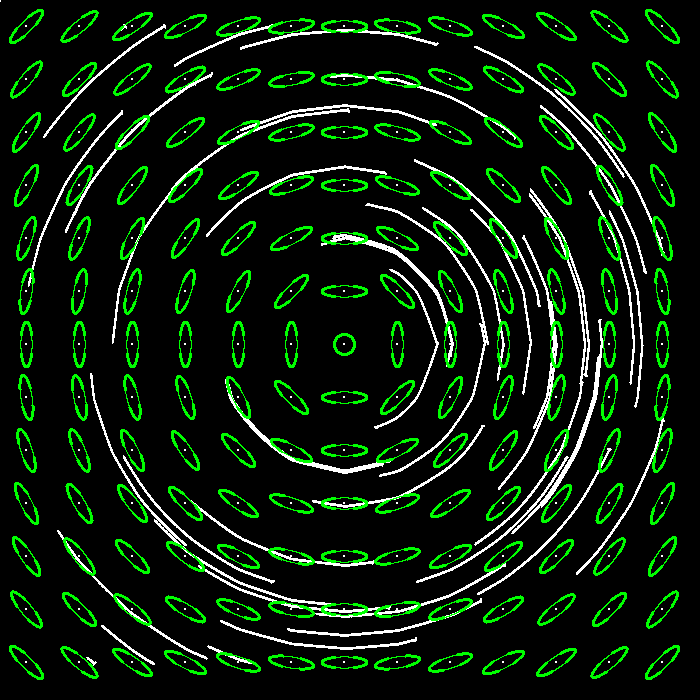
\includegraphics[width=0.5\textwidth]
    {img/tensorfieldlines.png}
  }
  \caption{white: bold lines; ellipsoids: ellipsoid glyphs}
  \label{scheme}
\end{figure}\vskip 3pt
Glyphs were derived as a basis for the weighting profiles of the tensors in the following propagation scheme. They were chosen because it is an easy-to-use (understand) concept which can also be interpreted nicely. In fact, these are used for the principal component analysis of direction vectors for the Tensor Field Line extrapolation (integration) in a subsequent step.
Tensor Field Lines (the type of tensor stream line - hyperstreamline analog that does not introduce artificial intertia) were implemented for Ground Truth (GT) data generation purposes. For example, when we design an FTLE-like field computation approach, we will need to know when tensor field lines diverge/converge.

\paragraph{Test Data (Generation)}
We used python's numpy library to generate pre-defined test cases and caught one real data example from \url{TensorVis.org}, which needed to be pre-processed through slicing and subsequent cropping to 2D samples ($2\times2$) matrices), which can be grouped into symmetric and asymmetric ones:\\

\begin{figure}[!t]
\centering
  \begin{minipage}{0.3\textwidth}
    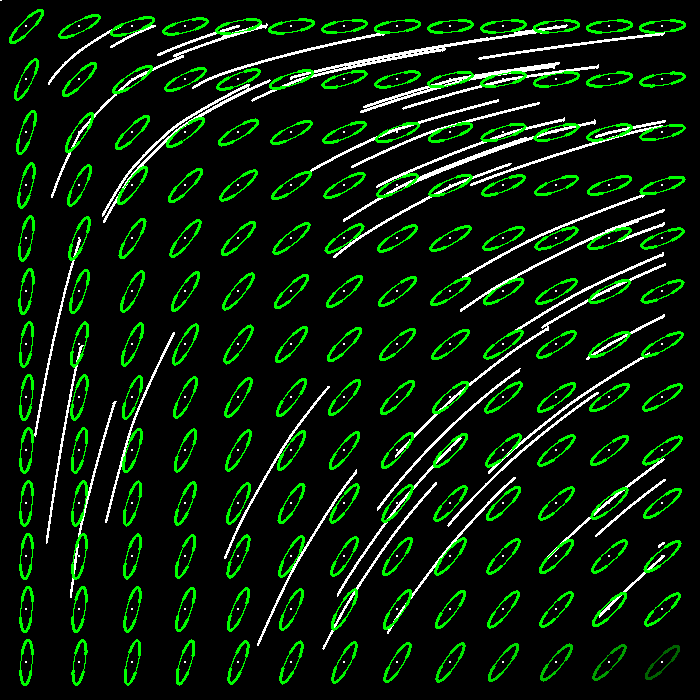
\includegraphics[width=\textwidth]{img/corner-TFL.png}
    \label{a)}
  \end{minipage}
  \begin{minipage}{0.3\textwidth}
    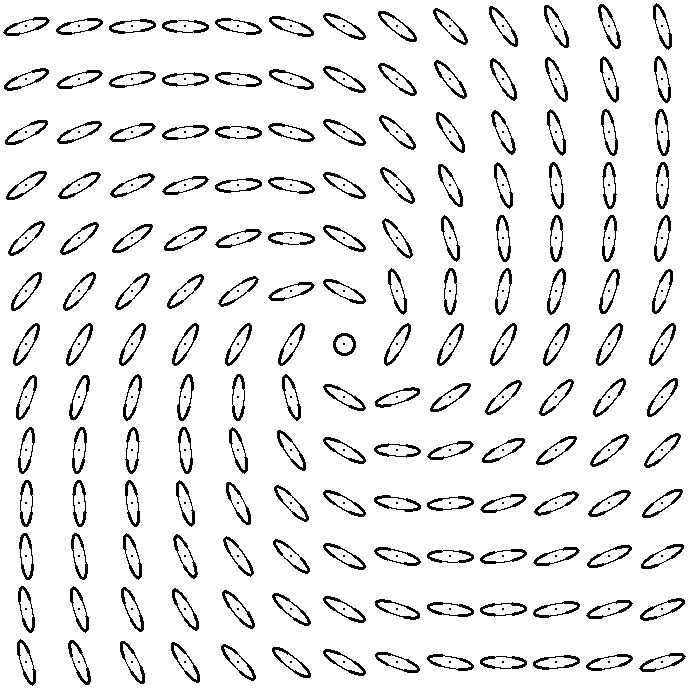
\includegraphics[width=\textwidth]{img/spiral.png}
    \label{b)}
  \end{minipage}
  \begin{minipage}{0.3\textwidth}
    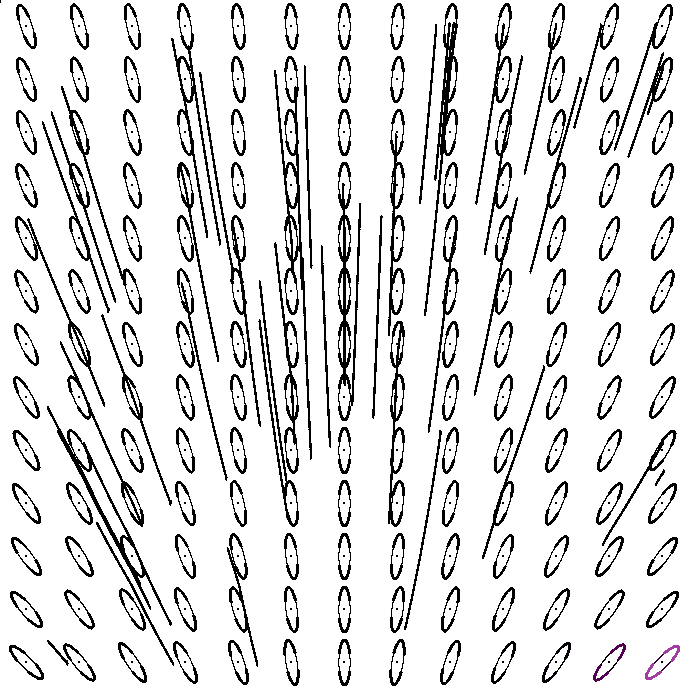
\includegraphics[width=\textwidth]{img/drain_old.png}
    \label{b)}
  \end{minipage}
\caption{a) ``corner''-Testfield, b) ``spiral''-Tesfield, c) ``V''-Tesfield}
\label{anisotropy}
\end{figure}

\textbf{Symmteric Tensor Fields}

\textbf{Asymmteric Tensor Fields}

\begin{figure}[!t]
\centering
  \begin{minipage}{0.4\textwidth}
    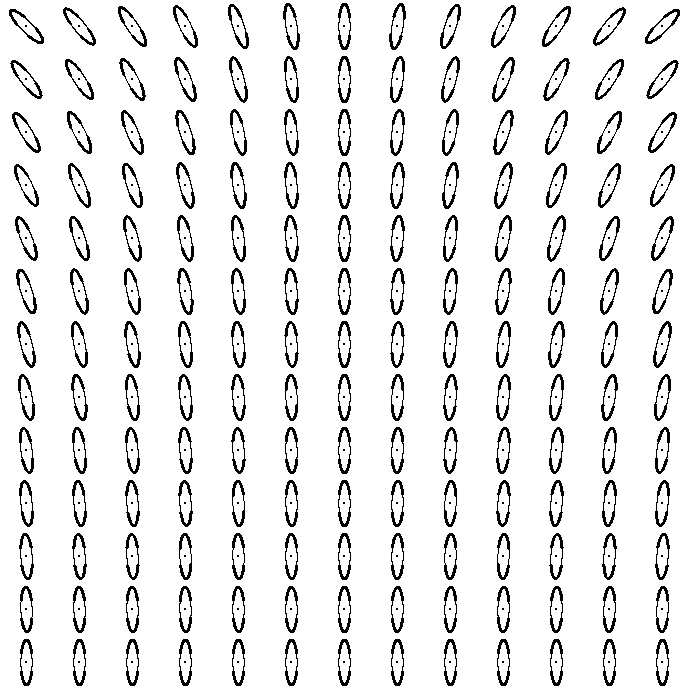
\includegraphics[width=\textwidth]{img/drain.png}
    \label{a)}
  \end{minipage}
  \begin{minipage}{0.4\textwidth}
    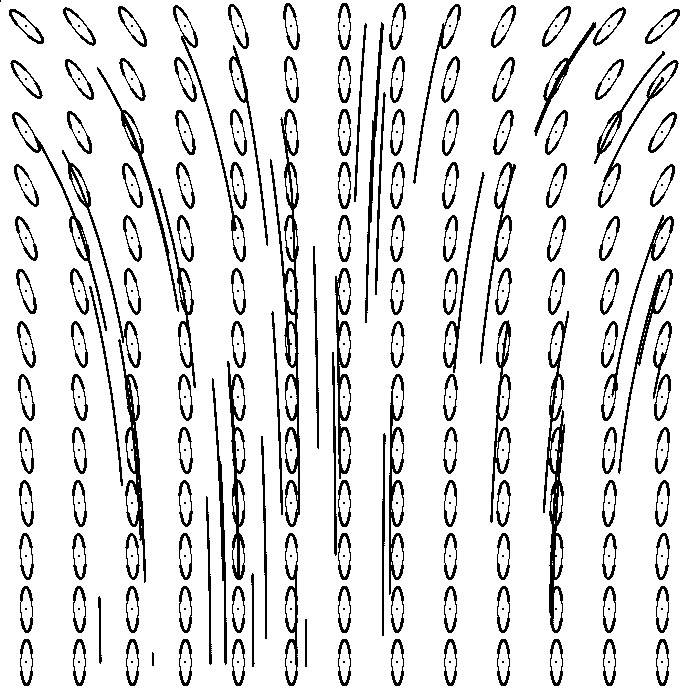
\includegraphics[width=\textwidth]{img/drain-TFL.png}
    \label{b)}
  \end{minipage}
\caption{a) ``drain''-testfield, b) tensor field lines for a)}
\label{anisotropy}
\end{figure}

The ``drain''-Testfield, depicted in Fig. \ref{drain} is generated to have a kind of proof-of-concept (POC) for the FTLE-related approach. It poses raw, bare diverging tensor field lines without any other feature modulated on top. Thus, it can be expected to induce a high FTLE response, since it is an interpretable ground truth test and is considered to be a basic trigger/stimulus for the approach.

\begin{figure}[!t]
\centering
  \begin{minipage}{0.4\textwidth}
    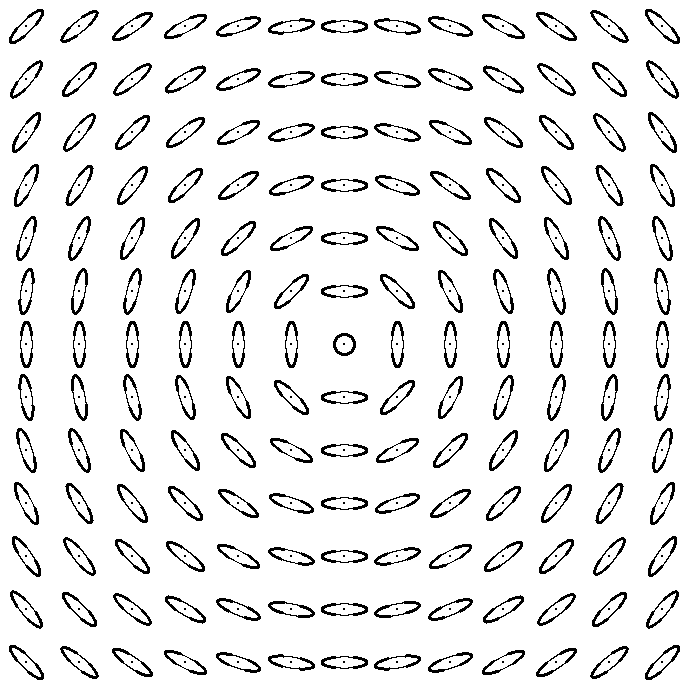
\includegraphics[width=\textwidth]{img/rings.png}
    \label{a)}
  \end{minipage}
  \begin{minipage}{0.4\textwidth}
    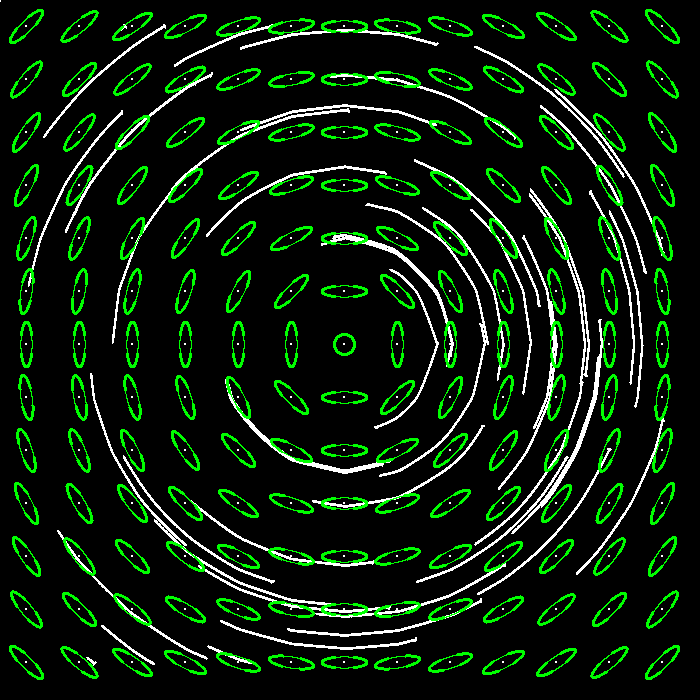
\includegraphics[width=\textwidth]{img/tensorfieldlines.png}
    \label{b)}
  \end{minipage}
\caption{a) ``rings''-testfield, b) tensor field lines for a)}
\label{drain}
\end{figure}

\begin{figure}[!t]
\centering
  \begin{minipage}{0.4\textwidth}
    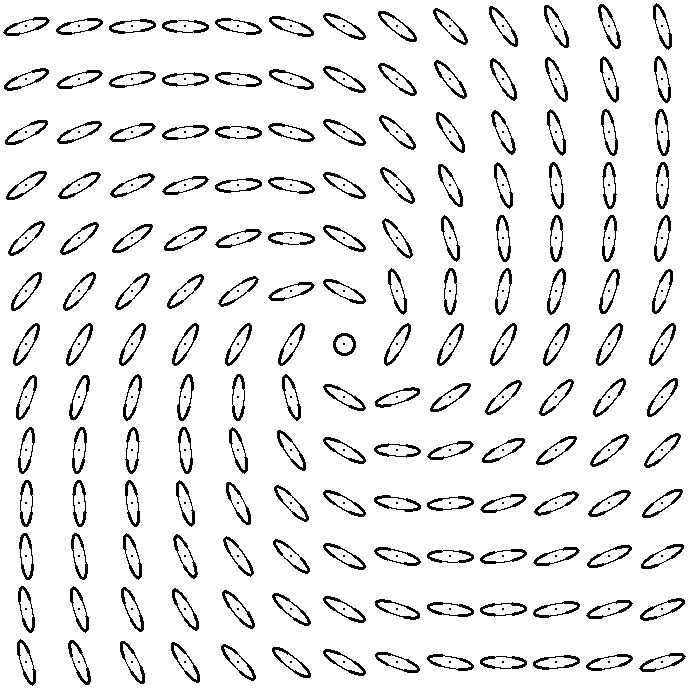
\includegraphics[width=\textwidth]{img/spiral.png}
    \label{a)}
  \end{minipage}
  \begin{minipage}{0.4\textwidth}
    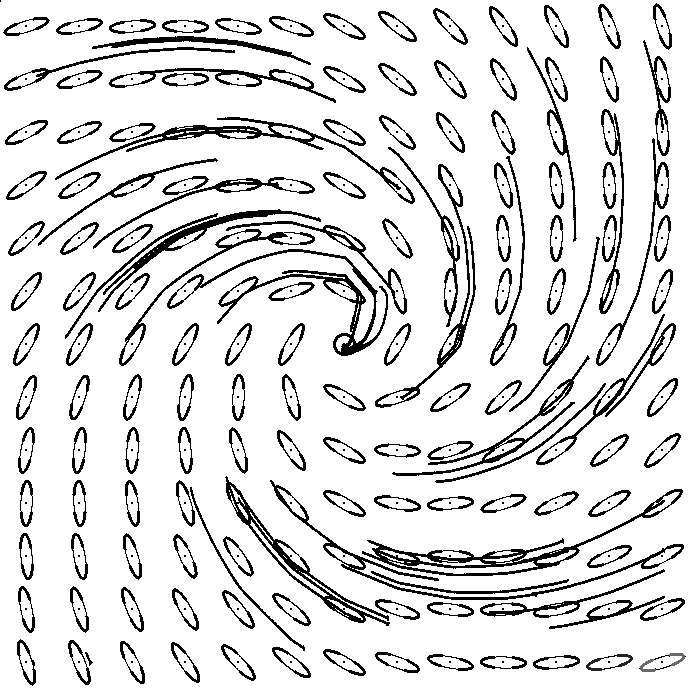
\includegraphics[width=\textwidth]{img/spiral-TFL.png}
    \label{b)}
  \end{minipage}
\caption{a) ``spiral''-testfield, b) tensor field lines for a)}
\label{spiral}
\end{figure}

\begin{figure}[!t]
\centering
  \begin{minipage}{0.4\textwidth}
    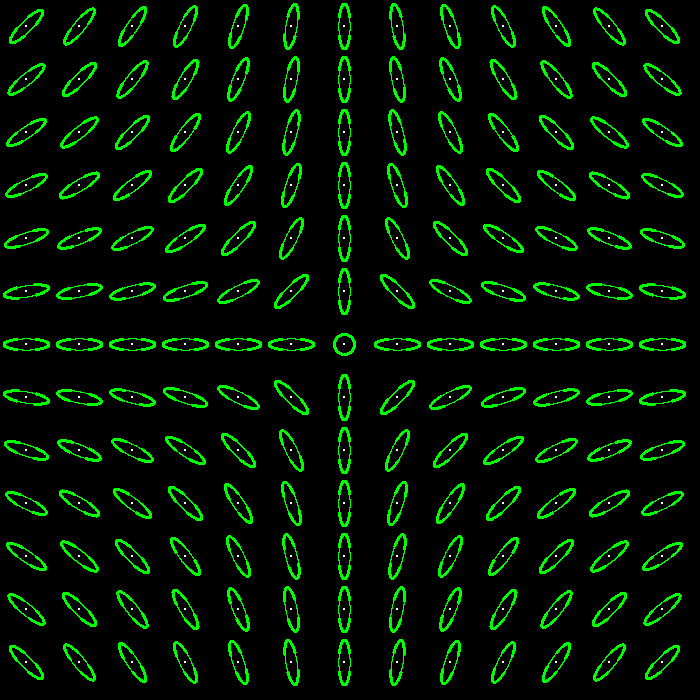
\includegraphics[width=\textwidth]{img/inverse.png}
    \label{a)}
  \end{minipage}
  \begin{minipage}{0.4\textwidth}
    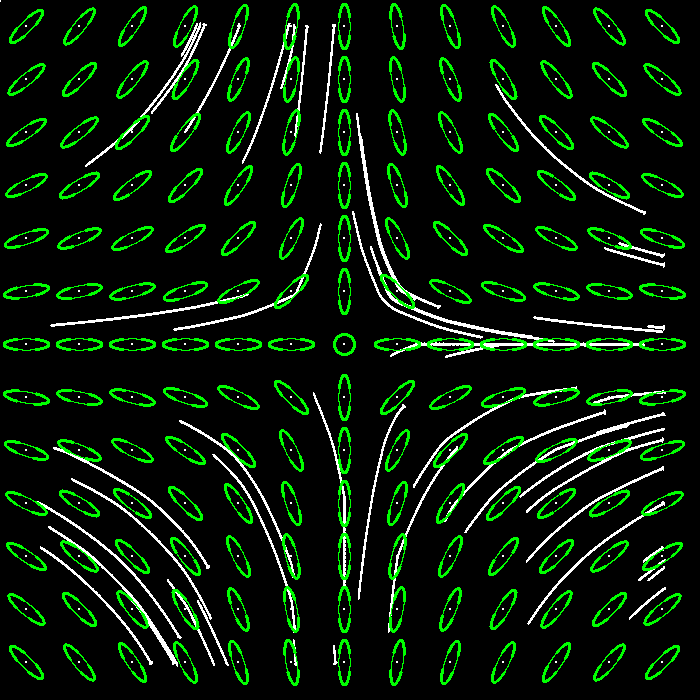
\includegraphics[width=\textwidth]{img/inverse-TFL.png}
    \label{b)}
  \end{minipage}
\caption{a) ``spiral''-testfield, b) tensor field lines for a)}
\label{spiral}
\end{figure}

\begin{figure}[!t]
\centering
  \begin{minipage}{0.4\textwidth}
    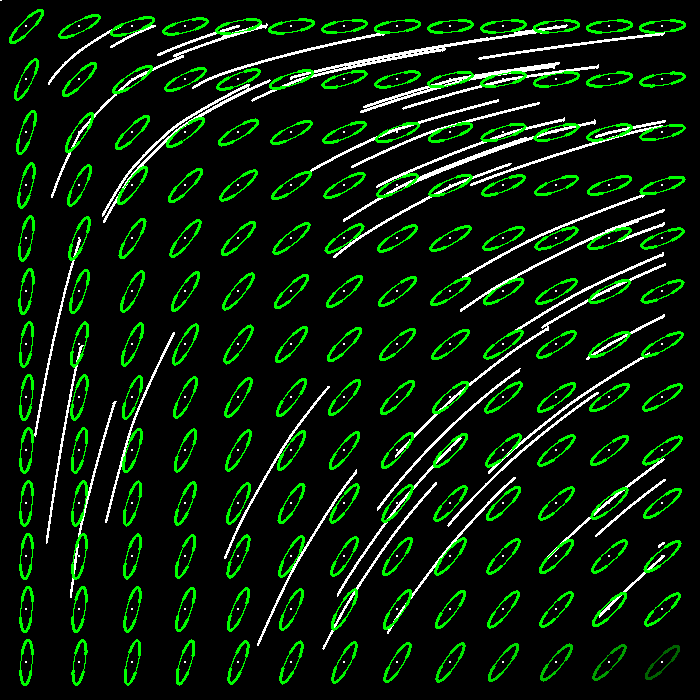
\includegraphics[width=\textwidth]{img/corner.png}
    \label{a)}
  \end{minipage}
  \begin{minipage}{0.4\textwidth}
    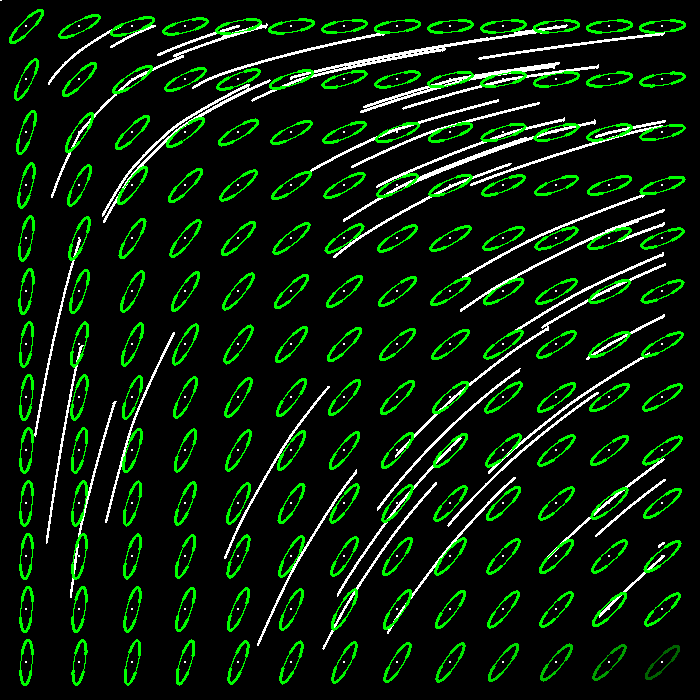
\includegraphics[width=\textwidth]{img/corner-TFL.png}
    \label{b)}
  \end{minipage}
\caption{a) ``corner''-testfield, b) tensor field lines for a)}
\label{spiral}
\end{figure}

\section{Related Work}
\label{sec:related}

There has been extensive recent work on symmetric tensors but in comparison little on asymmetric ones. Since we aren't able to cover the whole scope in this work, we will focus on the most relevant works on tensor field visualization. We will talk about the publications from Hlawatsch et al. \cite{hlawatsch} and Zirr et al. \cite{zirr} in particular, since they pose thematically related works.\vskip 5pt

\textbf{Symmetric Tensor Field Visualization}\\
Zheng \& and Pang \cite{pang&zheng} et al. proposed a texture-based visualization approach called HyperLIC, which extends the concept of LIC to symmetric tensor fields by using an anisotropic 2D-filter kernel oriented along the major/minor eigenvectors. The concept of following the major/minor eigenvector along tensor field lines was invented by Vilanova et al. \cite{vilanova}. Tensorlines introduce a kind of artificial inertia (running average), making them resistent to noise. The notion of tensor field topology and the concept of Hyperstreamlines was first introduced by Delmarcelle and Hesselink \cite{delmarcelle&hesselink}. The placement of tensor field lines as hyperstreamlines was recently improved by Spencer et al. \cite{spencer} for glyph packing. A good overview of seeding strategies concerning glyphs is given by McLoughlin et al. \cite{mcloughlin}. Feng et al. \cite{feng} used Voronoi Tesselation for placing the glyphs. Superquadric glyphs have been proposed by Schultz and Kindlmann \cite{schultz&kindlmann} for general (non-positive definite) tensors. De Leeuw and van Wijk \cite{deleeuw&vanwijk} visualize the partial derivative gradient, the Jacobian of the tensor field to sense the local properties of the field. A diffusion tensor can also be visualized by box \cite{makris}, ellipsoid \cite{pierpaoli}, composite \cite{westin2} or superquadric \cite{kindlmann} glyphs. There is also a set of scalar measures available in symmetric tensor field visualization such as: mean diffusivity, fractional anisotropy \cite{basser} and anisotropy coefficients \cite{westin}. Hlawatsch et al. \cite{hlawatsch} obtain a coordinate (flow) map from tensor field lines following major/minor eigenvectors (fibre trajectories) and use the maximum eigenvalue of the Cauchy-Green deformation tensor to compute the FTLE-field in homogeneous regions. In a similar manner, we aim to use light transport techniques to obtain a final light distribution through successive light propagation cycles footprinted (in form of transmission profiles obtained from ellipsoid glyphs) by the tensor field.
\\
\textbf{Asymmetric Tensor Field Visualization}\\
Zheng and Pang \cite{pang&zheng} proposed the concept of dual eigenvectors and Zhang et al. \cite{zhang} extended it to pseudo-eigenvectors and introduced the eigenvector/eigenvalue manifolds to visualize eigenvectors in the complex domain. Laramee et al. \cite{laramee} focused on the efficient implementation and visualization of these structures and provided an interactive visualization system for asymmetric tensors applicable in fluid and solid dynamics. The concept of Tensor Magnitude has been introduced by \cite{laramee2} for means of physical interpretation. They also proposed an efficient glyph and hyperstreamline hybrid approach, which made dynamic interaction in real-time in 2D tensor fields feasible. Palacios et al. \cite{palacios} extracted isosurfaces of tensor magnitude, mode and isotropy index. \vskip 5pt

Last, we will discuss our approach in relation to the listed publications. The FTLE-related approach ``global illumination gradient'' to be designed states a generalization of the light transport visualization method FTPD proposed by Zirr et al.\cite{zirr}, since it allows a similar measure to be computed through defining a geometrical scene and setting the transmission (tensor field) to an isotropic and constant value of $100\%$. In this modus, the approach operates as a light transport visualitation technique. The work of \cite{hlawatsch} et al. obtains similar results (an FTLE-like field) but obtains them by sampling of fiber trajectories instead of global illumination light transport methods, as in our case.
%Typischerweise im letzten Abschnitt dieses Kapitels wird dann auf
%verwandte Arbeiten eingegangen. Entsprechende Arbeiten sind geeignet
%zu zitieren. Beispiel: Die wurde erstmalig in den Arbeiten von Spitz
%und Gertz \cite{Spitz2016a} gezeigt \ldots Details dazu werden in
%dem Buch von Newman zu Netzwerken \cite{Newman2010} erl�utert \ldots.

%%%%%%%%%%%%%%%%%%%%%%%%%%%%%%%%%%%%%%%%%%%%%%%%%%%%%%%%%%%%
\newpage

% Alternative: put content in separate files
% Check the difference between including these files using \input{filename} and \include{filename} and see which one you like better
%\chapter{Einleitung}\label{intro}
%\input{introduction}
%
%\chapter{Voraussetzungen}\label{bg}
%\input{background}

%%%%%%%%%%%%%%%%%%%%%%%%%%%%%%%%%%%%%%%%%%%%%%%%%%%%%%%%%%%%
\newpage

\chapter{Method}
\label{chap:main}

This chapter will summarize the main contributions of this work studied and state targeted aims and goals as a first step in sect. \ref{sec:overview}. Then we will have a short introduction to the implemented global illumination scheme derived and simplified from an nVidia GI approach in sect. \ref{sec:scheme}. Last, we will state the effectively implemented Visualization methods Light Transport Visualization and Global Illumination gradient proposed as innovatively invented tensor visualization techniques.



%Dieses Kapitel stellt meist den Hauptteil der Arbeit dar. Vor dem
%ersten Abschnitt sollte ein kurzer �berblick (ein paar wenige S�tze
%mit Verweise auf nachfolgende Abschnitte) gegeben werden. Beispiel: Im
%nachfolgenden Abschnitt \ref{sec:overview} wir ein �berblick �ber die Anforderungen an
%das Modell gegeben. 

\section{Requirements and Ambitions}
\label{sec:spec} 
Our ambition is to motivate a simple and efficient global illumination propagation scheme able to distribute energy profiles in discrete polar form in 2D/3D-space w.r.t. energy conservation and propagation attenuation principles. We then generate transmission profiles from the eigensystems (principal component frames) of the tensors for each cell in the domain (field). That is, to provide an orientation for a grid of crystal fibre structures (cf. optical fibres) to redirect the intensities in analogy to the anisotropies of the tensor field within a glyph representation, obtained from Principal Component Analysis. Our approach should be implicitly adaptive to any kind of 2D dataset. Thus, we opt to be compatible to handle any kind of matrix (symm./anti-symm.) and any kind of resolution of the field (full-spectrum). At last, we aim to generate a new FTLE-related method for tensor field visualization by applying a Global Illumination Gradient to the resulting light distributions for every possible position and direction of the light source in the grid generated by stimulation with Delta-pulses. Thus, our motivation is to segment key locations (LCS/ridges) in the field with tensor field lines (hyperstreamlines) converging/diverging, which is necessarily the same (for bidirectional tensor fields). Our approach should efficiently handle (relatively) large datasets. 
%Knapp zwei Seiten, in dem die Anforderungen, die Zielsetzung und die
%Methoden �berblicksartig beschrieben werden. Hier sollte die
%Beschreibung ``technischer'' bzw.~``formaler'' sein als in der
%Einleitung, da der Leser nun mit den Grundlagen und verwandten
%Arbeiten vertraut ist.

\section{Global Illumination (Propagation) Scheme}
\label{sec:scheme}
Within the scope of this work, we will motivate a Global Illumination Scheme designed to efficiently propagate the intensities stored in discrete polar coordinates given as impulses (stimuli) by the user or the config. Polar profiles for different light sources are shown in Fig. \ref{polar}:
\begin{figure}[!t]
  \centering
 {
    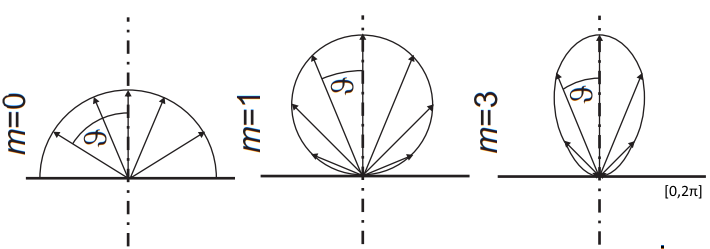
\includegraphics[width=0.8\textwidth]
    {img/strahler.png}
  }
  \caption{Polar profiles for different types of emitters ($m=0$: spherical emitter, $m=1$: Lambert emitter, $m=2$: cone emitter}
  \label{polar}
\end{figure}\vskip 3pt
As a reminder, polar profiles map each angle $\varphi$ a magnitude $r$ forming a function $r(\varphi)$. They are circular axis versions of the domain $[0..2\pi]$, with negative magnitudes mirrored by 180 degrees). Thus, they are functions with an angular domain making them directionally dependent, which is a well suited representation for point lights, as we use them in a style of Dachsbacher et al. \cite{dachsbacher}. For the sake of interpretability, we exclude negative values (energies) from the scope of our calculations. As a start-up thinker for the propagation scheme, we will think of a grid cell in 2D as a center pixel within an 8-neighborhood. Remember, that all considerations from now on are given concerning a single grid cell respectively. It has 8 (4 faces/edges and 4 diagonals) unique neighbors, which are adjacent point lights in the grid (the type of light source with theoretically no finite extend). We consider one face neighbor (top) to shortly explain the steps of the scheme. The diagonals and the others are obtained from derivation and symmetry.

Each cone (yellow and green) is an individual neighbor-dependent angular area. We optimize for distributing contributions for overlapping cones to transmit attenuated (because of the larger factor $\sqrt{2}$ distance) intensity in form of a shared part to the diagonals in a single step. Therefore, the intensity gathered in polar coordinates in areas marked in green, need to be partitioned between 2 of the 8 cone-index neighbors with following consideration:

\begin{figure}[!t]
  \centering
 {
    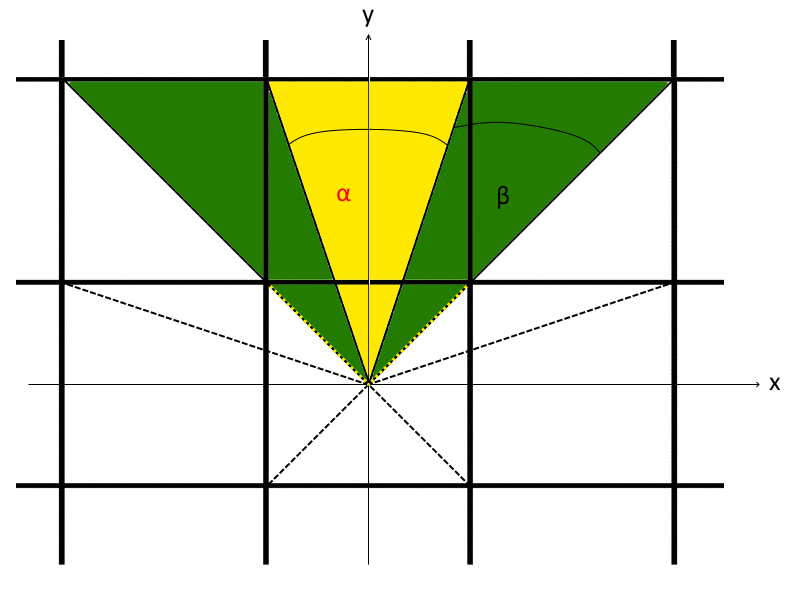
\includegraphics[width=0.8\textwidth]
    {img/scheme2.png}
  }
  \caption{Propagation Scheme}
  \label{scheme}
\end{figure}\vskip 3pt

The face neighbors take in the angular domain of $d_1=\alpha+2\beta$, whereas the diagonal neighbors span a domain of $d_2=2\beta$.
The linear combination weights for the overlapping (green) parts ($\beta$) are obtained from the relative overlapping angular area of the angular span $\beta$ w.r.t. diagonal cones ($2\beta$) and face cones ($\alpha+2\beta = 90^\circ$) (yellow cone is overlapped by green cones at full angle). The linear combination weights are subsequently normalized to $\sum = 1.0$ (normalization condition):
\begin{align}
	\varepsilon_1 &= \frac{\frac{\beta}{\alpha+2\beta}}{\frac{\beta}{\alpha+2\beta} + \frac{\beta}{2\beta}} \approx 0.362291\\
	\varepsilon_2 &= \frac{\frac{\beta}{2\beta}}{\frac{\beta}{\alpha+2\beta} + \frac{\beta}{2\beta}} \approx 0.63771.
\end{align}

We place a cosine lobe scaled with the integrated (accumulated) energies in each of the 8 cone directions, whereas outgoing integrated and summed energies are weighted by the linear combination weights (factors) in overlapping (green) areas to split up the contributions accordingly. The contribution areas are depicted in Fig. \ref{scheme}, the cosine lobes can be observed in Fig. \ref{iter} respectively. This manner of propagation is inspired by the propagation scheme of Dachsbacher et al. \cite{dachsbacher} (see the paper on how to ``project the flux into a point light''). The implementation is done in a dual buffer approach which pushes the energies back and forth (buffer A to buffer B) until convergence, which happens when the energy is spreaded throughout the grid and enters a stationary state, characterized by equal out (at grid borders) to in (at light source positions) energy-flow with no more nettings going on inside the domain. We measure the convergence criterion by setting up an overall distribution error w.r.t to the previous iteration. Note that even though we propagate the energy directly through the diagonal cones (which forms a square initially), the 8 degrees of freedom introduce a circular (spherical) wave front after few iterations (for greater resolutions) as depicted in Fig. \ref{iter}. This occurs, since the diagonals are more strongly attenuated by default and there is a redistribution of intensities in the long term resulting in a circular torus-shaped distribution, as observed in Fig. \ref{iter}. Also note, that this approach satisfies energy conservation and propagation attenuation principles and applies to the principles of light propagation in vacuum (by default). The verification of these principal requirements and specifications can be observed in the Experimental Evaluation in chap. \ref{chap:eval}.

We show a few of the first iteration steps for the propagation scheme in Fig. \ref{iter}:

\begin{figure}[!t]
  \centering
 {
    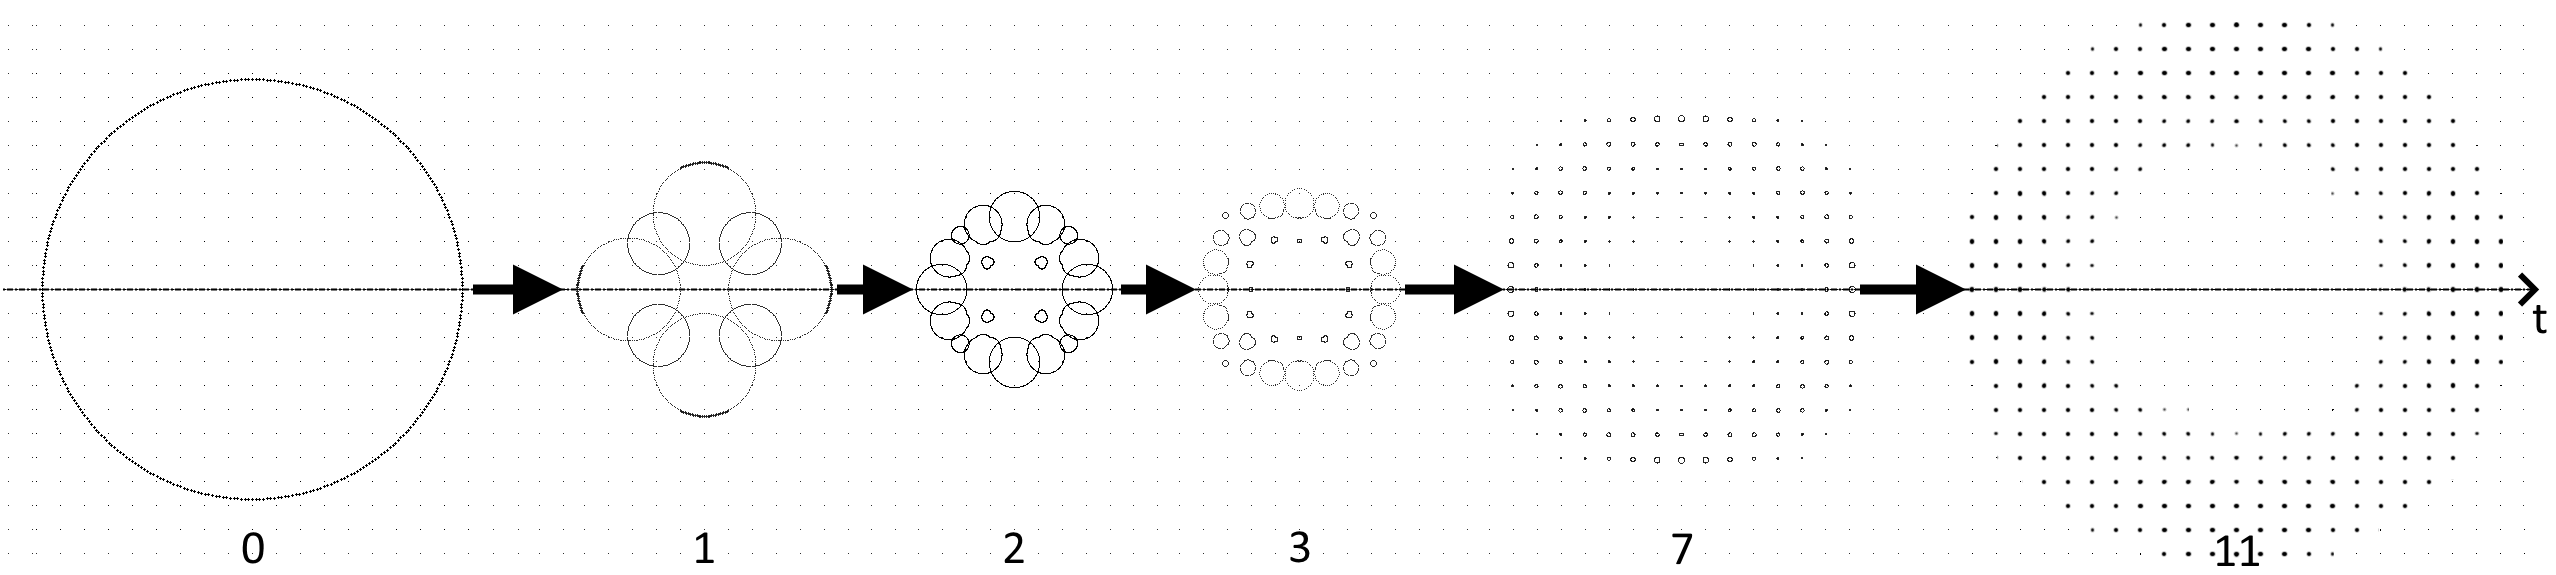
\includegraphics[width=1.0\textwidth]
    {img/steps_gallery_format_arrow_alt.png}
  }
  \caption{Impulse Response for Isotropic Stimulus (Few Iterations: 0,1,2,3,7,11)}
  \label{iter}
\end{figure}\vskip 3pt
Fig \ref{iter} depicts the named iteration inidices 0,1,2,3,7,11 for the propagation scheme for a circular pulse stimulus which gets turned off after 1 iteration to demonstrate raw energy spreading in the field (impulse response of algorithm). In step 1 one can observe the placing of cosine lobes scaled with the respective accumulated and weighted energy for the summed area in each of the 8 neighbor directions. In the subsequent steps, remark the evolution from an 8-neighborhood in step 1 to a circular torus shaped.

As already mentioned, a dual-buffer approach is chosen here, as we can efficiently propagate from one into the other and just swap pointers to 
start all over (after reinitialization) until convergence. Another reason is it yields a reasonable source-target structure. We introduce a new operator called \textit{propagate}, permitting us to pre-define the propagation in a symbolic manner. The propagation definition denotes the transformation from one grid (A-buffer) into another (B-buffer) through proper application of the \textit{propagate}-operator to each cell. We will fill this operator with meaning in sect. \ref{sec:trans} in form of a precise mathematical formulation respectively. Each Grid or Buffer is basically a set of cells defined as $\mathcal{C} = \{\mathbf{c}_1, \mathbf{c}_2, ..., \mathbf{c}_i\}$.  The dual buffer result $\mathcal{C'}$ is denoted symbolically as follows for all cells with a mean intensity greater than zero (which do not contain trivial Null samples):
\begin{align}
	\mathcal{C'} = \mathop{propagate}\{c_i\in \mathcal{C} \ \mid \ |\mean{I}_i| > 0\} \hskip 5pt {\forall } \ i \in [1,\mathop{dim}].
\end{align}
The dual buffer result $\mathcal{C'}$ denotes the set of all transformed cells after the propagation after applying the operator $\mathop{propagate}$ to each cell. This result is generated once in each iteration and gets pushed back and forth between the 2 buffers. Note that, $\mathop{dim}=width\cdot height$, which equals the tensor field resolution in this case and remark that wedenote the final buffer result $\mathbf{b}=\mathcal{C}_{final}$ in the following. At last, we define a threshold for the minimum overall distribution error taken into account for convergence conditions, initiating a stop sequence when falling below that threshold $\epsilon$ (, e.g., $0.5$) :\\
\paragraph{Criterion:}
\begin{align}
	\Delta I_{sum} = \sum_{i\in\mathcal{C}}  \Delta I_i(\omega) \overset{!}{<} \epsilon.
\end{align}


Until now, we aimed to simulate the propagation of light in empty space (vacuum) providing us with a physically-motivated but very simplified base-approach. We aim to modulate the transmission of the intensities on top of the base approach with transmission profiles obtained from the tensor fields through principal component analysis, which yields ellipsoid glyph equations in the following.


%In diesem und den nachfolgenden Abschnitten werden die Beitr�ge der
%Arbeit motiviert, formal sauber (oft mathatisch, sprich mit
%Definitionen etc.) beschrieben, und bei Bedarf mithilfe von Beispielen
%verdeutlicht. Die Beschreibungen in diesem Kapitel sind meist
%unabh�ngig von einer konkreten Realisierung und Daten; diese werden im
%nachfolgenden Kapitel detailliert.

\section{Transmission Profiles and Weighting Functions}
\label{sec:trans}
To obtain a kind of footprint of the tensor field, we set up ellipse equations for each glyph representation, obtained from applying PCA on each cell (tensor) in the field. Concurrently, we construct our abstract mathematical operator \textit{propagate}, previously referenced in  We map the singular values (corresponding to eigenvalues) in decreasing order to the ellipses radii (half-axes) $a(\lambda_1 )$ and $b(\lambda_2 )$ as follows:

Ellipse Equation:
\begin{align}
	r(\omega) = \frac{ab}{\sqrt{a^{2}\sin^{2}(\omega-\varphi)+b^{2}\cos^{2}(\omega-\varphi)}} =\frac{\lambda_1\lambda_2}{\sqrt{\lambda_1^2\sin^2(\omega-\varphi)+\lambda_2^2\cos^2(\omega-\varphi)}}.
\end{align}
That is, the singular values form the half-axes of the PCA ellipsoid, which yields us a symbolic definition for our transmission (transfer) function as weighting profiles. We compute the offset angle $\varphi$ w.r.t. x-axis by exploiting the atan2-function with 4-quadrant evaluation for the first singular vector. As a preliminary prep, this profile is precomputed (sampled) for all discrete angular steps for each cell (, e.g., $360$). The weighting scheme which we apply is depicted in Fig. \ref{weighting}.
\begin{figure}[!t]
  \centering
  {
    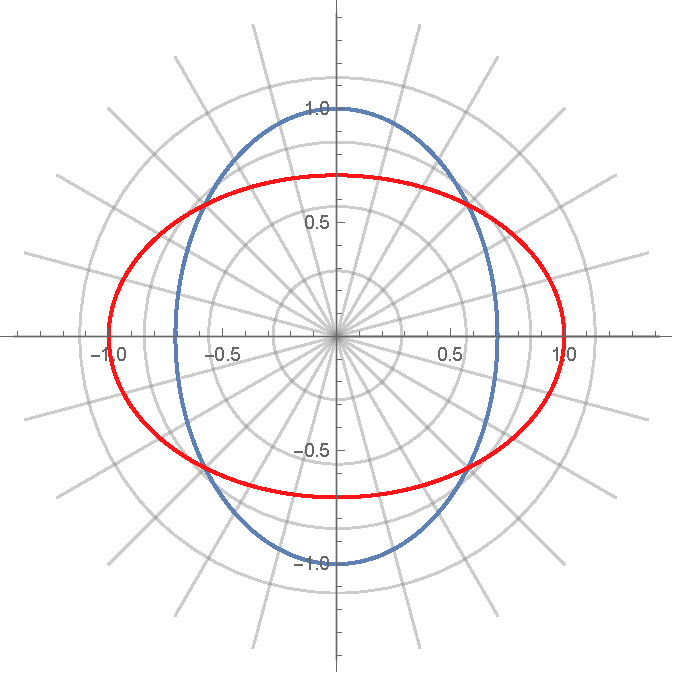
\includegraphics[width=0.6\textwidth]
    {img/polarplot.pdf}
  }
  \caption{red: Intensity Profile, cyan: Transmission Profile (glyph Ellipsoid Eq.)}
  \label{weighting}
\end{figure}
We interpret the polar functions as discrete, sampled 1D vectors with a uniform angular resolution. That means, we use element-wise multiplication for the 1D-vectors in red (Intensity Profile) and cyan (Transmission Profile) to obtain a windowed version of the intensity profile and perform the following integration step to accumulate the total radiant power (flux) as follows. Note that we model angular dependent radiant intensity ${I}(\omega) [\frac{W}{\mathop{rad}}]$ as an underlying physical entity, which is well suited for describing point light sources. As a side note, the physical quantity perceived as brightness by human eyes, is the radiance (luminance), which is yielded by relating radiant intensity to a finite sensitive area ($[\frac{W}{\mathop{rad}}/m^2]$). The primary definition for our total accumulated incident radiant flux (presuming that the cone is given in local coordinates - i.e. centered around the origin) is then denoted as:

\begin{align}
	\Phi_{t,\alpha} &= \int_{-\pi/4}^{\pi/4}{T}(\omega){I}(\omega)\mathop{d\omega}\\
	\Phi_{t,\beta} &= \int_{-\beta}^{\beta}{T}(\omega){I}(\omega)\mathop{d\omega}\\
	\sum_{\cos_+} &= \int_{-\frac{\pi}{2}}^{\frac{\pi}{2}}\cos_+(\omega)\mathop{d\omega} \approx 2.
\end{align}

This permits us to scale an oriented and clipped cosine-lobe $\cos_+$ with the total radiant flux w. respect to its own total energy when integrated likewise. A discrete cosine lobe never reaches its theoretical sum of $2$ exactly in the interval $[{-\frac{\pi}{2}},{\frac{\pi}{2}}]$. Therefore it needs to be computed to account for floating-point precision errors and normalized by following relation (, e.g., $\sum_{\cos} \approx 1.9949204635834517$).
\begin{align}
	\cos_n(\omega) = \frac{\Phi_t}{\sum_{\cos}}cos(\omega).
\end{align}
This yields a cosine lobe, which has an overall energy of $\Phi_t$ if the point light is interpreted with a Lambert-emitter (cf. \cite{lindlein}) characteristic (as part or area element of a diffusely reflecting surface) since the intensity profile matches a cosine in this case. 

Now each tensor ellipse equation has a mean transmission rate $[\%]$, which turns out to be a measure or synonym for the total rate of the outgoing transmitted radiant intensity $\int_0^{2\pi}{T}(\omega)\mathop{d\omega}$. Since energy can not be generated from transmission profiles (only transmitting, not generating), we have to normalize every tensor ellipse equation with the highest mean transmission rate in the field, which is then transmitting the whole outgoing intensity $\int_0^{2\pi}{I}(\omega)\mathop{d\omega}$. This restricts the tensor ellipse mean to a maximum of $100\%$ for the one with the highest tensor magnitude. We will use the definition of mean tensor magnitude $\mean{r}_{max}$ obtained from the PCA here for simplicity. Hence the tensor ellipse equations are normalized through the following step:
\begin{align}
	r_n(\omega) = \frac{1}{\mean{r}_{max}}r(\omega).
\end{align}
Notice, that this implements the concept of absorption implicitly, because tensors with a lower mean $\mean{r}$ than $100\%$ lose energy wheras absorption equals ${\mu} = {1}-{\mean{r}}$ here. Now that we have coped with the problem of overall transmission, we are left with another problem that occurs with the weighting functions as they can still yield values above $1.0$. This would potentially generate intensity out of nothing which leads to crucially unstable behaviour. Well, but only in case energy conservation principles were not respected.  To construct a solution, we ask for the source of the excessive energy. If the tensor mean complies with the constraint $\mean{r}\leq 1.0$, then the energy must lack in some other place (since the overall transmission fulfills the energy conservation constraint in that case). The only problem is that a normalization condition in usual style for the transmission profile ${T}(\omega)$ does not necessarily imply the same normalization for the term ${T}(\omega){I}(\omega)$. However, a proper normalization can provide corrective support, wich reveals another subsequent normalization constraint. The normalization factor is defined in 3 subsequent steps:
\begin{enumerate}
	\item Normalization of $TI$ to $\overline{TI}=1.0$
	\item Subsequent scaling w. mean intensity $\mean{I}$ for energy conservation principles
	\item Subsequent scaling w. mean tensor magnitude $\mean{T}$ for absorption principles
\end{enumerate}

Hence the transmitted energy is given as:

\begin{align}
	{I}_t(\omega) &= n_f{T}(\omega){I}(\omega) \hskip 30pt w. \ n_f = \frac{\mean{T}\mean{I}}{\overline{TI}}.
\end{align}

This transforms our equation for the radiant flux into:
\begin{align}
	\Phi_{t,i} &= \int_0^{2\pi}{T}_i(\omega){I}_{t,i}(\omega)\mathop{d\omega}.
\end{align}
Which is now respecting energy conservation principles very conveniently, as all we need is a set of means and we are done. This collapses our abstract mathematical operator $\mathop{propagate}$ applied to each cell into the following steps:
\begin{enumerate}
	\item Computation of normalization factor $n_f$
	\item Direction (component)-wise weighting to account for shared part in diagonal cones
	\item Integration (accumulation) total radiant flux weighted with transmission profiles inside the angular neighbor range (read-access)
	\item Scaling of cosine lobe corresponding to neighbor direction and subsequent placing to corresponding neighbor (write-access)
	
\end{enumerate}

This approach ensures that no energy will be generated and therefore implements the 	physical law of energy conservation or Kirchhoff's current law if you want to think of a particle's diffusion process. Consequently, this allows us to assume that all sources of power (energy) are user-defined. In fact the approach has proven to be robust w.r.t. energy losses for several iterations as depicted in chap. \ref{chap:eval} in the stochastic error graph.

\section{Physical Model}
\label{sec:model}
To pose a physical interpretation for the transmission of the tensor field, we imagine a melting crystal with  fibrous structures aligning with the major eigenvectors of the tensor field. This is what we call the footprint of the tensor field. This can be observed in, e.g., the gemstone tiger's eye cat's eye effect, where crystal fibers align with the crystal axes respectively. The propability density function $P(\omega)$, for a photon being scattered in a particular direction $\omega$ \ref{ryder}, is then described as:
\begin{align}
 	P(\omega) &= \frac{T(\omega)}{\int_{k\pi}^{(k+1)\pi}T(\omega)\mathop{d\omega}}\\
 	w. \int_0^{2\pi} P(\omega) &= 1.
\end{align}
This propability density function (PDF) indicates whether there is directed anisotropy or spherical isotropy w.r.t the neighboring $180$ ($\pi \mathop{rad}$ degrees.

\section{Global Illumination Gradient}
\label{sec:ftle}
Now, that we are able to propagate intensity in grid, directed by the eigenvectors of the tensor field, we aim to do something more elaborate to segment ROIs (regions of interest) characterised by divergence/convergence of tensor field lines and drastic changes in anisotropy. We opt to extract ridges from this FTLE-like field to grasp the key regions separating anisotropy behavior in the field, which are in turn LCS (Lagrangian Coherent Structures) well known for their rich substance in physical meaning. They can even be observed in nature for, e.g., vortices in flow fields. For that, we will use our, previously defined $\mathop{propagate}$-operator on every possible light source location $\mathbf{x}$ and direction $\omega$ in the grid to obtain the set of buffers $\mathcal{B} = \{\mathcal{C}_1, \mathcal{C}_2, ..., \mathcal{C}_j\}$:
\begin{align}
	\mathcal{B} = \mathop{propagate}\{c_i\in \mathcal{C} \ \mid \ |\mean{I}_i| > 0\} \ {\forall } \ i \in [1,\mathop{dim}] \ {\forall } \ j \in [1,\mathop{dim}\cdot \mathop{steps}].
	\label{ftle}
\end{align}
Whereas $j$ is the index of light source position and direction representing the initialization in each iteration and $\mathop{steps}$ is the count of the discrete angular steps. The initialization is done by placing a light src (delta-impulse) with $\mean{I}_i = 1.0$ at the exact location of index $j$ realizing a light source at location $(x\mid y)$ in direction $\omega$. Eq. \ref{ftle} now denotes the set of buffers $\mathcal{B}$ containing light distributions propagated from every possible direction and location. Now, that we have measured impulse responses from every location in our long 1D sample vector, we can incorporate finite (central) differences to obtain the Gradient of the set of final buffers with elements $\mathcal{C}_{final}=\mathbf{b}\in\mathcal{B}$:
\begin{align}
	\nabla \mathbf{b}_{x,y,\omega} =
	\begin{pmatrix}
	\frac{\partial \mathbf{b}_{x,y,\omega}}{\partial x} \\ \frac{\partial \mathbf{b}_{x,y,\omega}}{\partial y} \\ \frac{\partial \mathbf{b}_{x,y,\omega}}{\partial \omega}
	\end{pmatrix} \approx
	\frac{1}{2}
	\begin{pmatrix}
	\sum_{\mathbf{c}}\lvert \mathbf{b}_{x+1,y,\omega} - \mathbf{b}_{x-1,y,\omega}\rvert \\ \sum_{\mathbf{c}}\lvert \mathbf{b}_{x,y+1,\omega} - \mathbf{b}_{x,y-1,\omega}\rvert \\ \sum_{\mathbf{c}}\lvert \mathbf{b}_{x,y,\omega+1} - \mathbf{b}_{x,y,\omega-1}\rvert
	\end{pmatrix} =
	\frac{1}{2}
	\begin{pmatrix}
	\sum_{\mathbf{c}\in \mathbf{b_x}}\lvert \mathbf{b_x}\rvert \\ \sum_{\mathbf{c}\in \mathbf{b_y}}\lvert\mathbf{b_{y}}\rvert \\ \sum_{\mathbf{c}\in \mathbf{b_{\omega}}}\lvert \mathbf{b_{\omega}}\rvert
	\end{pmatrix}.
\end{align}
 
Note that this step is very expensive considering runtime-costs since it follows the following runtime observation. We have $\mathop{width}\cdot \mathop{height}\cdot \mathop{steps}$ numbers in the grid and on top $\mathop{width}\cdot \mathop{height}\cdot \mathop{steps}$ buffers in total, which need to be processed. Also we remark the convergence criterion which introduces another factor $\mathop{width}$ and set $\mathop{height}=\mathop{width}$ here for simplicity, which yields:
\begin{align}
	\mathcal{O}(\mathop{width^5}\mathop{steps^2}).
\end{align}
It is noticeable that the runtime increases fast with increasing resolution, which makes parallelization algorithms a crucial tool to compute the results in reasonable time. Next, we compute the Euclidean norm of the Global Illumination Gradient yielding a scalar field, which can be visualized directly or via extracted ridges in ParaView from VTK format:
\begin{align}
	\lvert\nabla \mathbf{b}_{x,y,\omega}\rvert = \sqrt{(\frac{\partial \mathbf{b}_{x,y,\omega}}{\partial x})^2 + (\frac{\partial \mathbf{b}_{x,y,\omega}}{\partial y})^2 + (\frac{\partial \mathbf{b}_{x,y,\omega}}{\partial \omega})^2}.
\end{align}
Note that the resulting scalar field is $(n+1)$-dimensional ($x,y$ and direction $\theta$) and needs to be flattened by averaging or projection in 3D for proper visualization in case the approach will be adopted. 

%%%%%%%%%%%%%%%%%%%%%%%%%%%%%%%%%%%%%%%%%%%%%%%%%%%%%%%%%%%%
\chapter{Experimental Evaluation}
\label{chap:eval}
\section{Propagation Attenuation}
\label{sec:att}
It can be proven that the approach follows propagation attenuation principles and follows the inverse (square) law ($\sim\frac{1}{r}$) as observed in the graph in Fig. \ref{att}. For that, we plot the relative intensity $i_{rel}(r_{rel})$ (in relation to the intensity at position (radius) $1$ to account for the inverse square law, which holds for relative distances. We evaluate the relative intensity by forming a ratio $\frac{I(r)}{I_1}$, that relates the step intensity to the src intensity at position 1.

\begin{figure}[!t]
  \centering
 {
    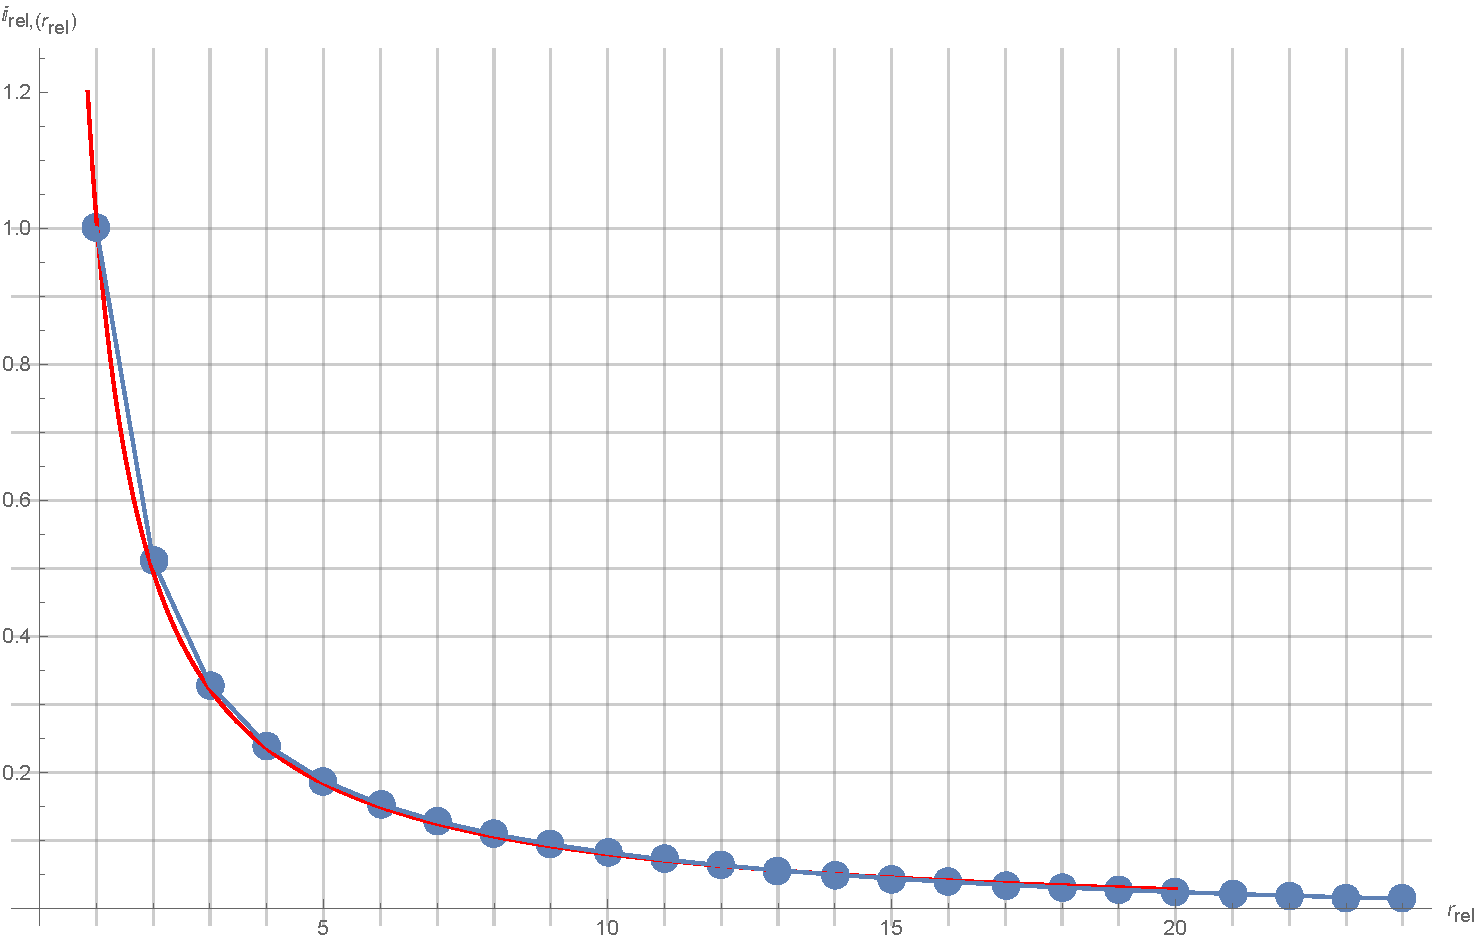
\includegraphics[width=0.7\textwidth]
    {img/inverse_law.pdf}
  }
  \caption{Propagation Attenuation}
  \label{att}
\end{figure}\vskip 3pt

\section{Light Propagation Scheme Behaviour}
To evaluate the plausibility of the light distribution results obtained from the light propagation scheme, we plot the transmission profiles overlaid with the resulting intensity profiles for several synthetic test fields:
\begin{figure}[!t]
\centering
  \begin{minipage}{0.4\textwidth}
    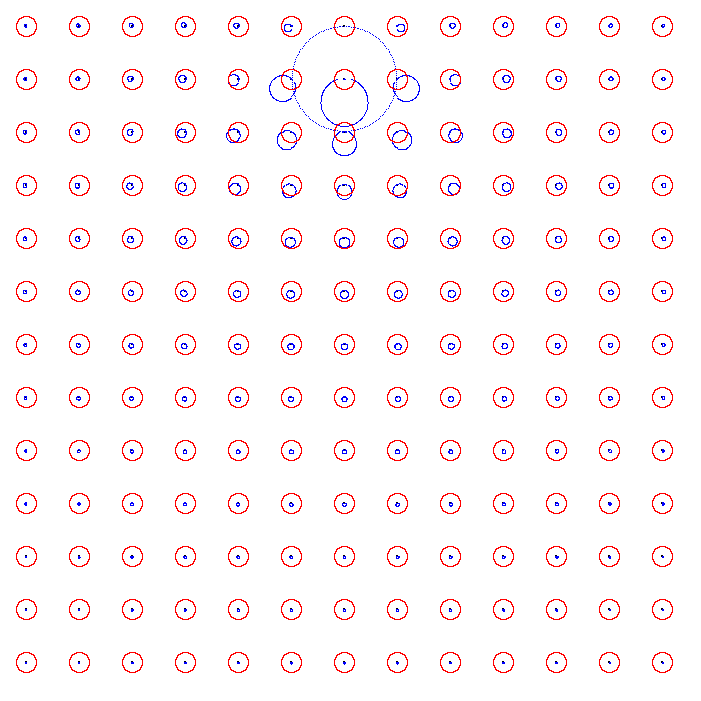
\includegraphics[width=\textwidth]{img/isotropic.png}
    \label{a)}
  \end{minipage}
  \begin{minipage}{0.4\textwidth}
    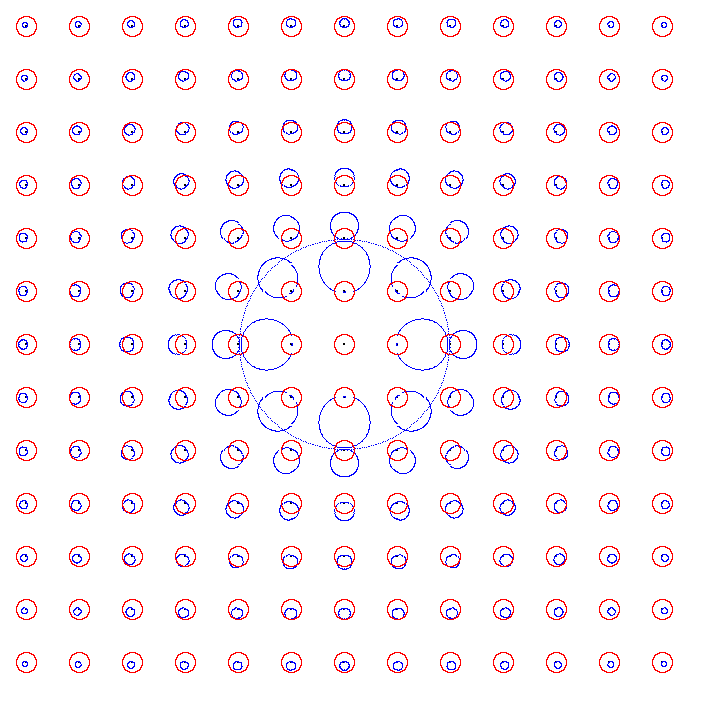
\includegraphics[width=\textwidth]{img/isotropic-all-center.png}
    \label{b)}
  \end{minipage}
\caption{final light propagation distributions for ``isotropy''-testfield}
\label{isotropic}
\end{figure}

\begin{figure}[!t]
\centering
  \begin{minipage}{0.4\textwidth}
    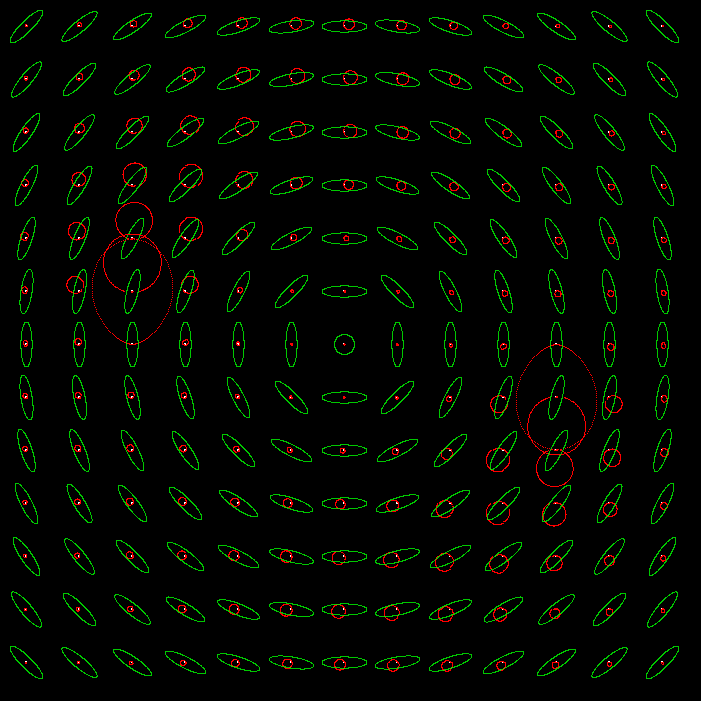
\includegraphics[width=\textwidth]{img/rings-two-special1.png}
    \label{a)}
  \end{minipage}
  \begin{minipage}{0.4\textwidth}
    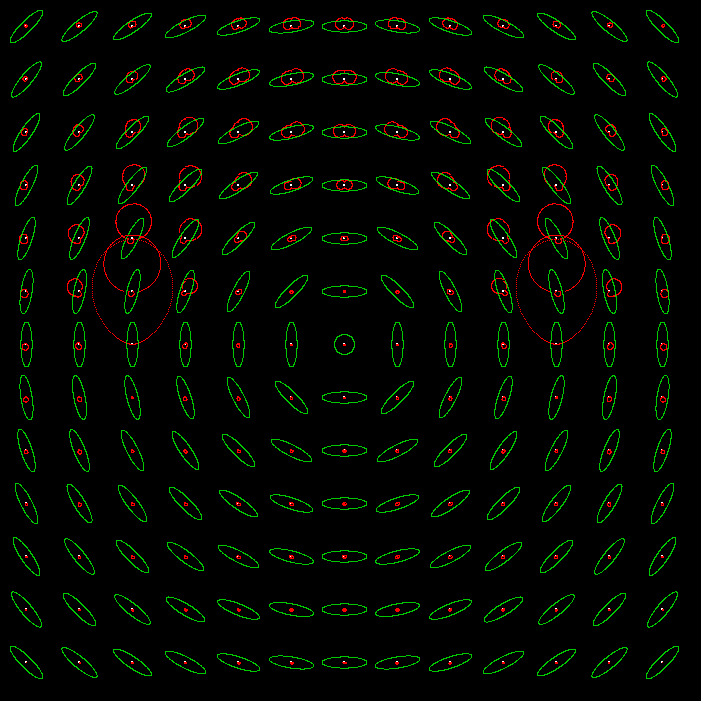
\includegraphics[width=\textwidth]{img/rings-two-special2.png}
    \label{b)}
  \end{minipage}
\caption{final light propagation distributions for ``rings''-testfield}
\label{rings-tests}
\end{figure}

\begin{figure}[!t]
\centering
  \begin{minipage}{0.4\textwidth}
    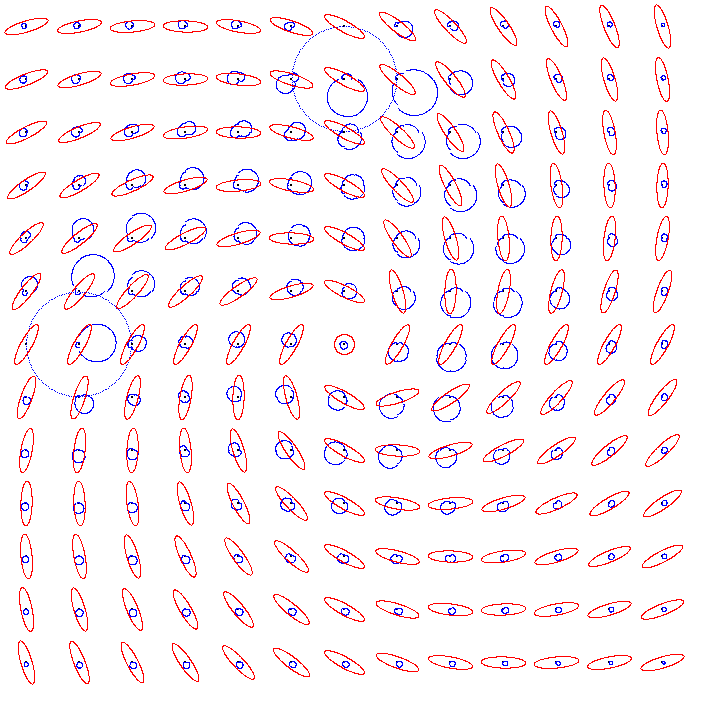
\includegraphics[width=\textwidth]{img/spiral-two-dense.png}
    \label{a)}
  \end{minipage}
  \begin{minipage}{0.4\textwidth}
    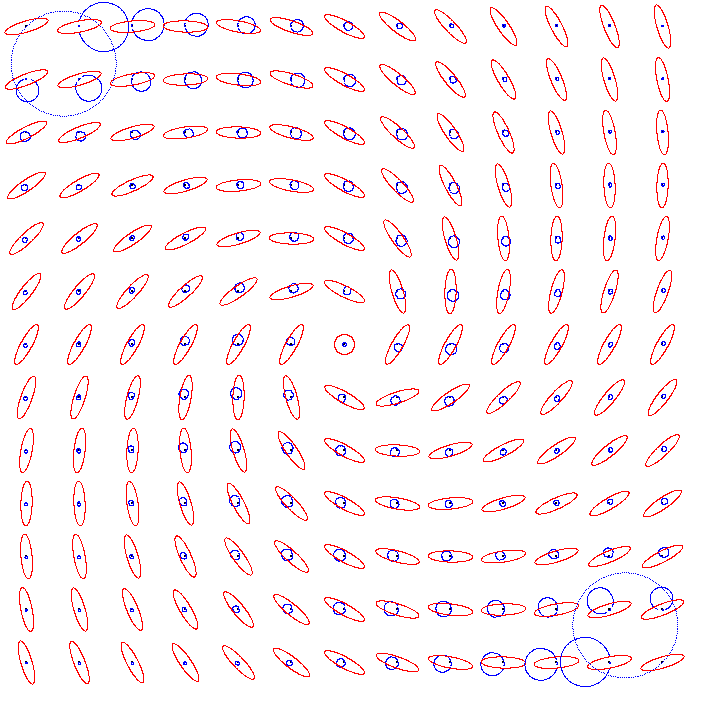
\includegraphics[width=\textwidth]{img/spiral-two-wide.png}
    \label{b)}
  \end{minipage}
\caption{final light propagation distributions for ``spiral''-testfield}
\label{spiral-tests}
\end{figure}


\begin{figure}[!t]
\centering
  \begin{minipage}{0.33\textwidth}
    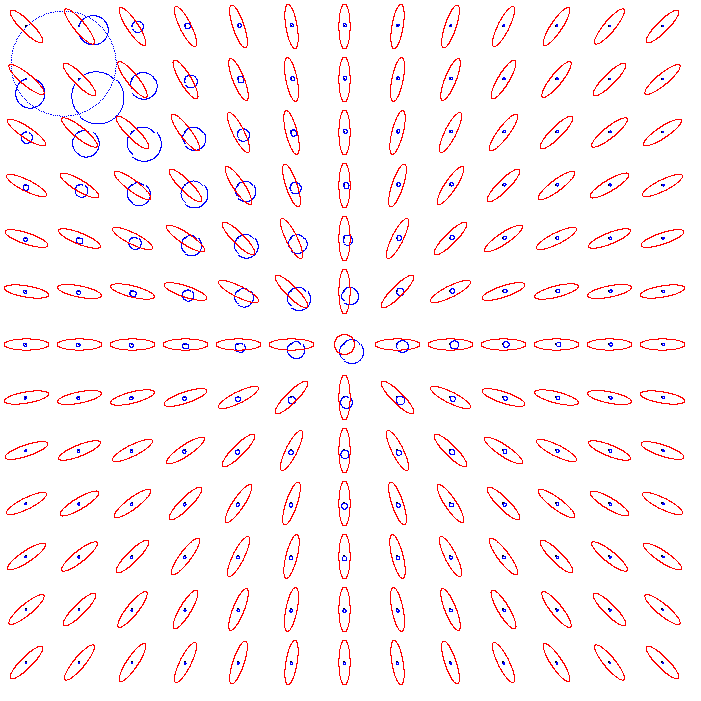
\includegraphics[width=\textwidth]{img/star-0,0.png}
    \label{a)}
  \end{minipage}
  \begin{minipage}{0.33\textwidth}
    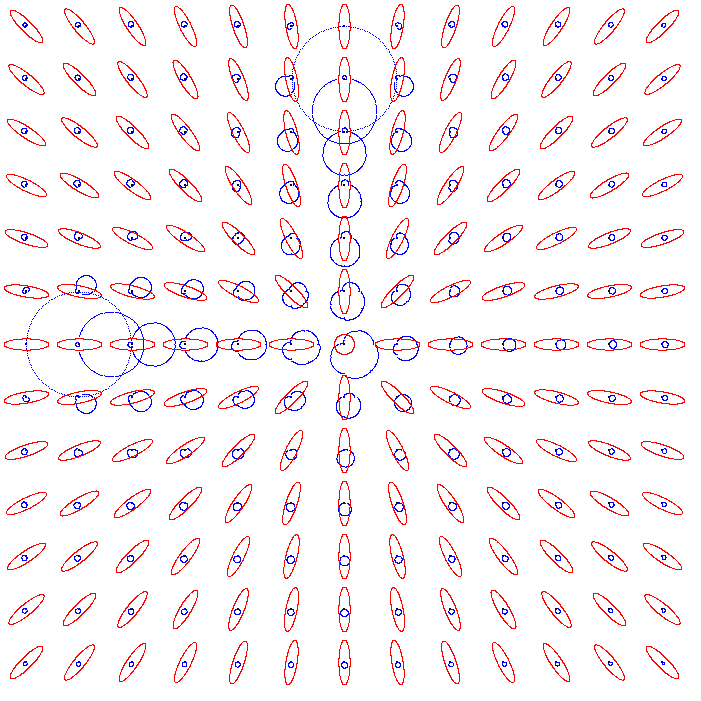
\includegraphics[width=\textwidth]{img/star-two-dense.png}
    \label{b)}
  \end{minipage}
   \begin{minipage}{0.33\textwidth}
    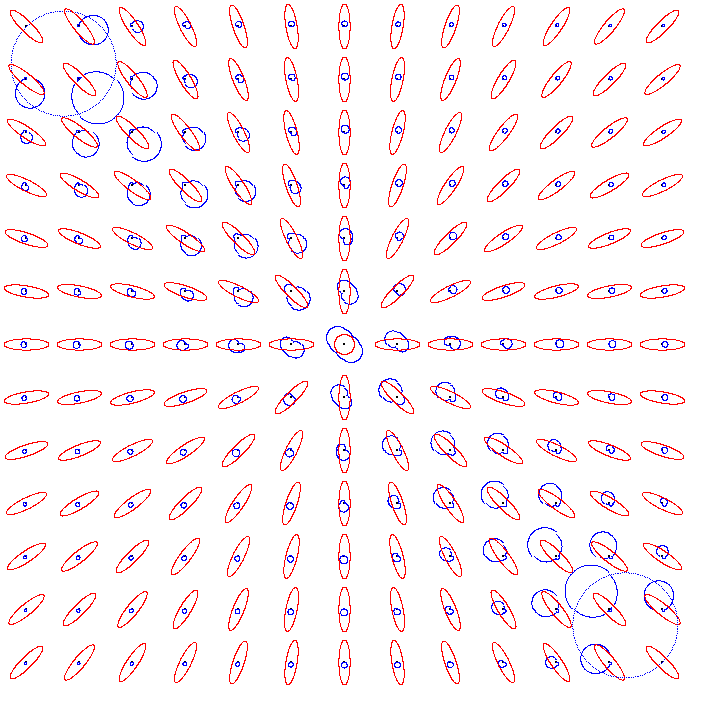
\includegraphics[width=\textwidth]{img/star-two-wide.png}
    \label{c)}
  \end{minipage}
\caption{final light propagation distributions for ``star''-testfield}
\label{spiral-tests}
\end{figure}

\section{Behaviour for Total Anisotropy}
We also wanted to check for the limitations of the approach by having total linear anisotropy (the case whereas one eigenvalue $\lambda_1>0$ and the other $\lambda_2=0$) incorporated. For this we set up bidirectional delta-pulses as glyphs to have the whole energy transmitted in just one, discrete direction.
\begin{figure}[!t]
\centering
  \begin{minipage}{0.4\textwidth}
    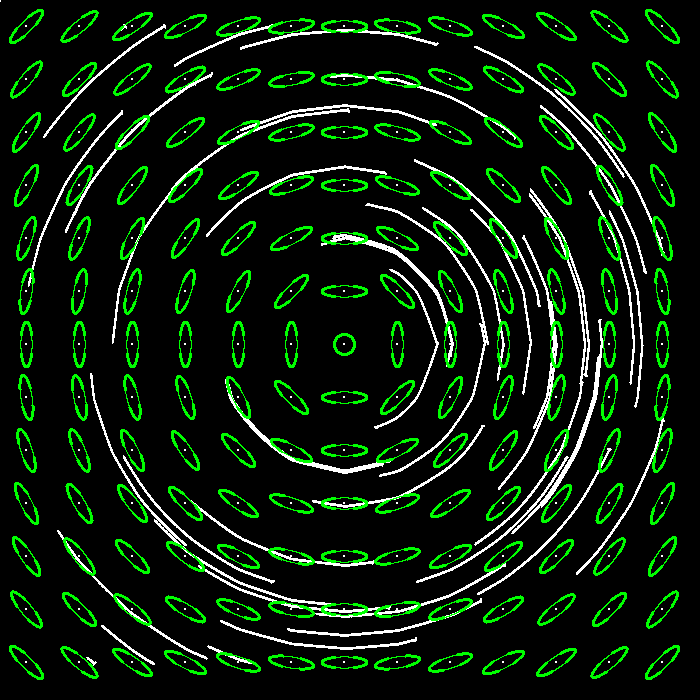
\includegraphics[width=\textwidth]{img/tensorfieldlines.png}
    \label{a)}
  \end{minipage}
  \begin{minipage}{0.4\textwidth}
    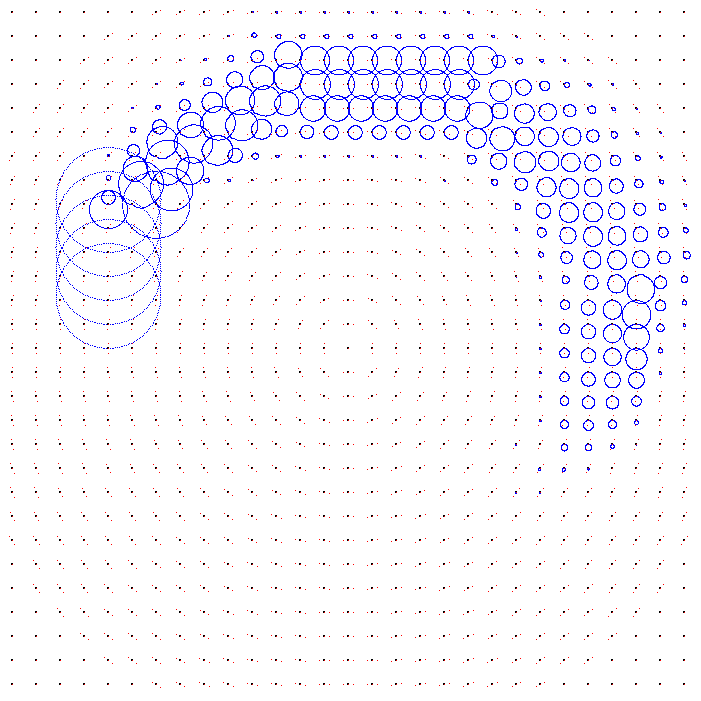
\includegraphics[width=\textwidth]{img/total_anisotropy.png}
    \label{b)}
  \end{minipage}
\caption{a) tensor field Lines and glyphs for ``rings''-Testfield, b) intensity propagation in grid}
\label{anisotropy}
\end{figure}
What we can observe here, is kind of a sampling drift as the approach uses 8 discrete directions to propagate averaged intensity whereas the circle uses much more (namely infinite). Hence, the energy can never follow a perfect circle, but at best an 8-edged octagon. This means, that there is a drift of at least two cells per diagonal (one overshoot per enter/escape each) as observable in Fig. \ref{anisotropy}.
\section{Energy Conservation Test}
The Energy Conservation Test was done in similar manner as the Propagation Attenuation Test in sect. \ref{sec:att}. We measure the impulse response of the algorithm for about 80 iterations by summing the total energy in the grid after each iteration and comparing it to the initial energy sum in iteration 0 in absolute values. This approach yields the following graph:

\begin{figure}[!t]
  \centering
 {
    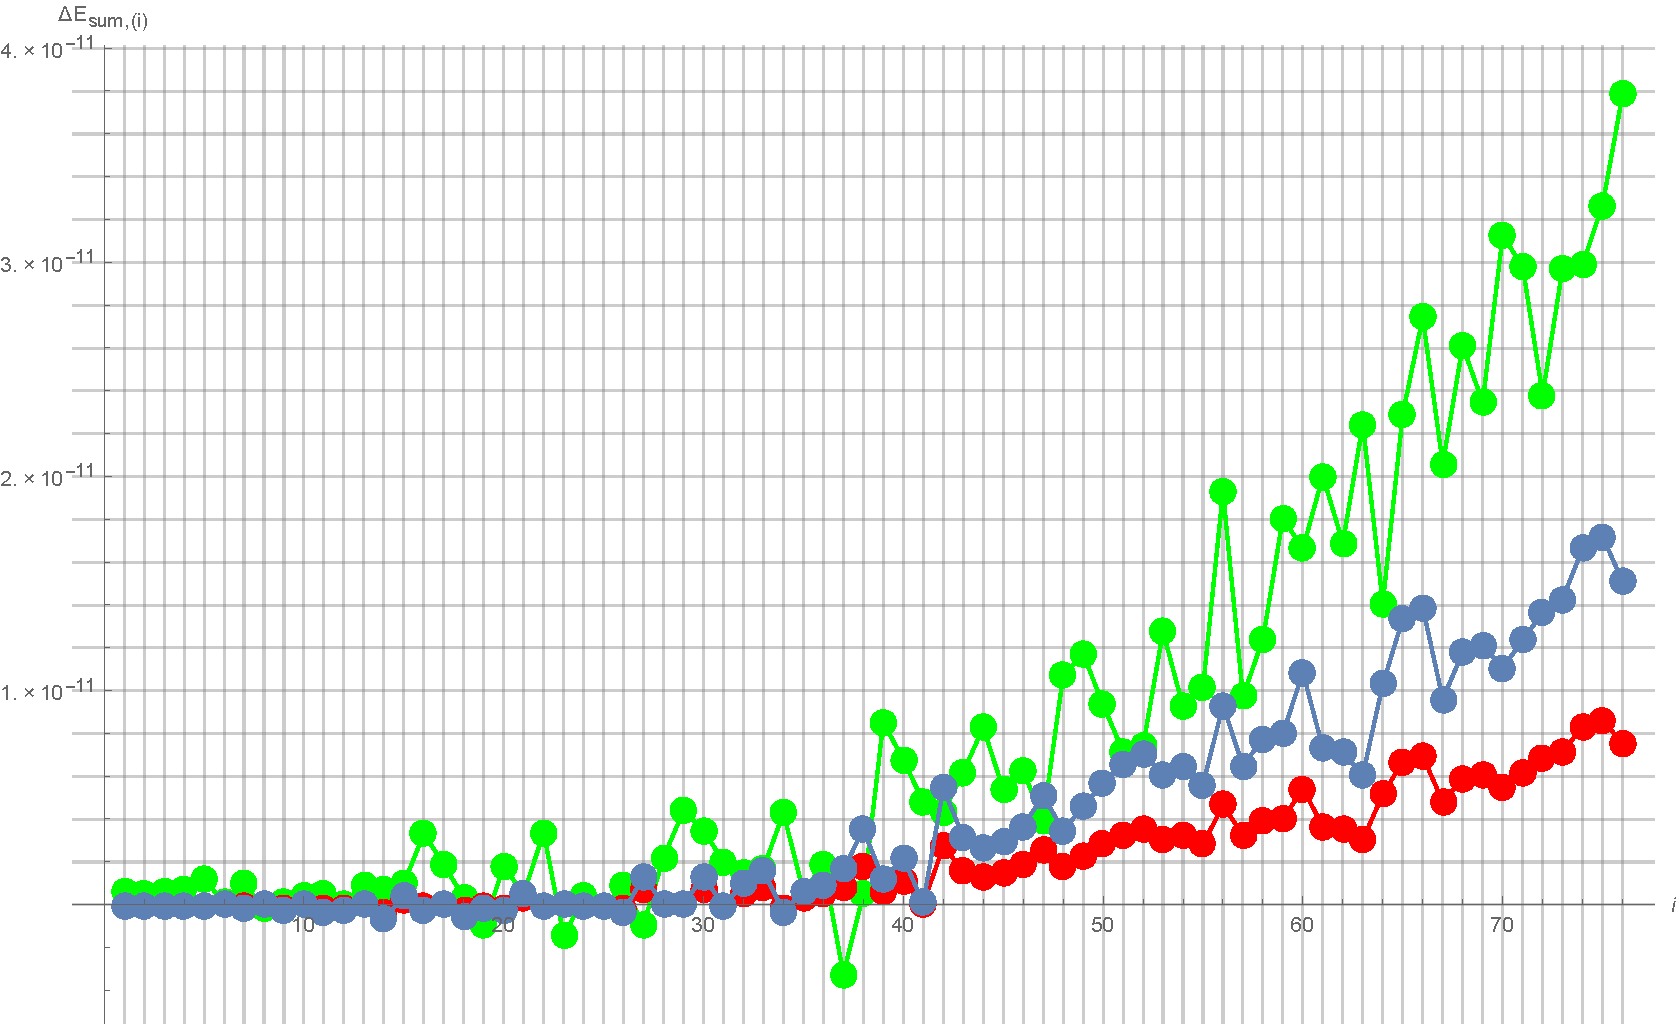
\includegraphics[width=0.7\textwidth]
    {img/sum_difference.pdf}
  }
  \caption{Sum Error: src intensities: red: 1.0, blue 2.0, green: 5,0}
  \label{anisotropy}
\end{figure}

The approach remains stable until iteration 40, which is at the time (point) when the numbers are to small and get rounded down under the double machine epsilon. You can see heavy fluctuations because the numbers get rounded upwards likewise. But what is lost, is lost and can not be gained back. The error is accumulating gradually and with faster slope for higher source intensities, since floting point precision, i.e., rounding errors operate more heavily on large numbers leading to a greater absolute $\Delta E$

\section{Light Transport Gradient (LTG)}
The light transport gradient approach, which is closely related to the FTLE approach in vector fields is evaluated from simple ground truth examples to elaborate real datasets.
As a little warmup, we will have an experiment exhibting bare, raw tensor field lines diverging w.r.t. one axis.
\begin{figure}[!t]
\centering
  \begin{minipage}{0.4\textwidth}
    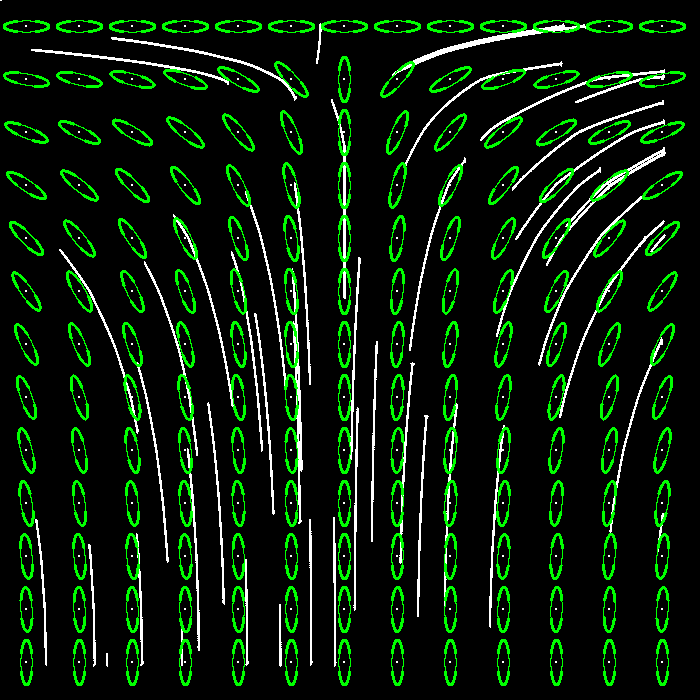
\includegraphics[width=\textwidth]{img/drain(alt)-TFL.png}
    \label{a)}
  \end{minipage}
  \begin{minipage}{0.4\textwidth}
    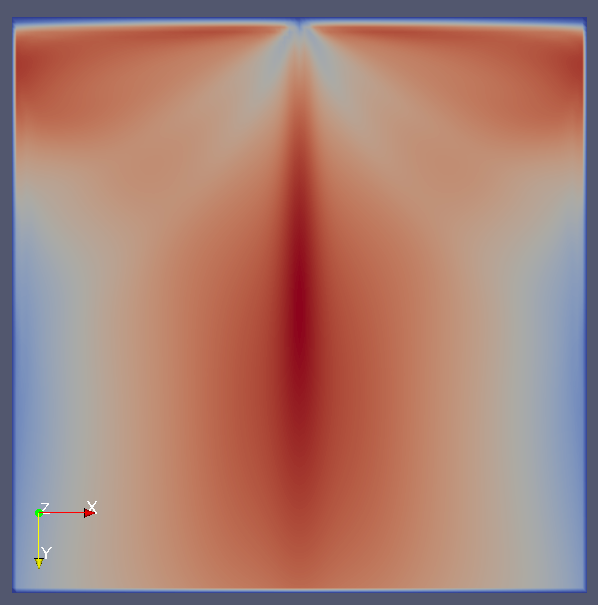
\includegraphics[width=\textwidth]{img/ftle_drain_alt.png}
    \label{b)}
  \end{minipage}
\caption{a) tensor field lines and glyphs for ``drain''-Testfield, b) LTG for a)}
\label{anisotropy}
\end{figure}
What we can observe here, is called a ``ridge'' occuring as a high value line segment (red vertical track) with edges amplified by a gradient filter. These ridges represent ROIs with underlying Lagrangian coherent structures, which we already discussed in sect. \ref{sect:motiv}.

\section{temp}
Der Aufbau dieses Kapitels oder dessen Aufteilung in zwei Kapiteln ist
stark von dem Thema und der Bearbeitung des Themas
abh�ngig. Beschrieben werden hier Daten, die f�r eine Evaluation
verwendet wird (Quellen, Beispiele, Statistiken), die Zielsetzung der Evaluation
und die verwendeten Ma�e sowie die Ergebnisse (u.a.~mithilfe von
Charts, Diagrammen, Abbildungen etc.)

Dieses Kapitel kann auch mit einer Beschreibung der Realisierung eines
Systems beginnen (kein Quellcode, maximal Klassendiagramme!).

%%%%%%%%%%%%%%%%%%%%%%%%%%%%%%%%%%%%%%%%%%%%%%%%%%%%%%%%%%%%
\chapter{Zusammenfassung und Ausblick}
\label{chap:concl}

Hier werden noch einmal die wichtigsten Ergebnisse und Erkenntnisse
der Arbeit zusammengefasst (nicht einfach eine Wiederholung des
Aufbaus der vorherigen Kapitel!), welche neuen Konzepte, Methoden und
Werkzeuge Neues entwickelt wurden, welche Probleme nun (effizienter)
gel�st werden k�nnen, und es wird ein Ausblick auf weiterf�hrende
Arbeiten gegeben (z.B.~was Sie machen w�rden, wenn Sie noch 6 Monate
mehr Zeit h�tten).


% References (Literaturverzeichnis):
% a) Style (with abbreviations: use alpha):
% see
% https://de.wikibooks.org/wiki/LaTeX-W%C3%B6rterbuch:_bibliographystyle
% for the different formats and styles

\bibliographystyle{ieeetr} %acm - as capital letter ALTERNATIVE
% b) The File:
\bibliography{references}

\end{document}
